\documentclass{article}
\usepackage{geometry}
\usepackage{amsmath}
\usepackage{amsfonts}
\usepackage{amssymb}
\usepackage{amsthm}
\usepackage{tikz}
\usepackage{hyperref}

\title{\textbf{Pythagorean Triples, etc.}}
\author{\scshape{Fred Barnes}\\ \href{mailto:fredlb@centurytel.net}{\texttt{fredlb@centurytel.net}}}
\date{2008--04--29}

\renewcommand{\labelenumi}{\roman{enumi}.}

\usetikzlibrary{angles,quotes}

\newtheorem{theorem}{Theorem}
\newtheorem{lemma}{Lemma}
\newtheorem{corollary}{Corollary}
\theoremstyle{definition}
\newtheorem{claim}{Claim}
\newtheorem{example}{Example}[section]
\newtheorem{case}{Case}[section]
\renewcommand{\theexample}{\arabic{section}\Alph{example}} 
% Changes example numbering to say "Example 1A." instead of "Example 1.1."
\renewcommand{\thecase}{\arabic{case}} % This just changes the style so that it says "Case 1" instead of "Case 1.1" where the number comes from the section number.

\pagenumbering{roman}

\begin{document}

\begin{titlepage}
\maketitle

\begin{abstract}
Observations on Pythagorean triples, on the solutions of 120 degree and 60 degree integer-sided triangles, and on deriving complex numbers from the law of cosines.
\end{abstract}

\tableofcontents

\clearpage

\section*{Preface}
\label{sec:Preface}
\addcontentsline{toc}{section}{\protect\numberline{}Preface}
% This section should not have a number but should still be in the TOC. From https://tex.stackexchange.com/questions/222959/adding-the-preface-to-contents

This document is a PDF transcription of \url{http://pythag.net/triples.html}. However, the site has long gone. You can view an online version on a GeoCities archive at \url{http://www.geocities.ws/fredlb37/node23.html} (advertisement warning), or a snapshot on the Internet Archive at \url{https://web.archive.org/web/http://www.pythag.net/triples.html}. While the snapshot at the Internet Archive is newer (updated 2010), not all pages were archived: including a section titled ``Hubble". Alas, this document transcribes the 2008 version, as indicated on the title page.

The webpages were generated with \texttt{LaTeX2HTML}, which is now quite outdated (although still functional). While Barnes does provide PDF files for some individual sections, it would be more convenient to condense it into one document.

I have rearranged some sections, since Barnes has clearly written some of the more complex ones before he decided to expand on their preliminaries, and made them their own page. These preliminaries are now shown before their relevant section. However, as a result, there are a lot of ideas and phrases repeated in this document (especially the formulae in Section 1).

I still included Barnes' email address on the title page, though to save you  time, that email address is no longer available; you will recieve a message stating \texttt{550 5.1.1 [R2] Recipient} \texttt{fredlb@centurytel.net does not exist here.} You can still get in touch with me, the transcriber, on my GitHub account at \url{https://github.com/Infiaria}.

\bigskip

\noindent\textbf{Notation}
\begin{itemize}
\item \(|x|\) is the absolute value of \(x\).
\item \(\equiv\) means ``equivalent to".
\item \(a \equiv b \pmod{c}\) means that the remainder of \(a\) when divided by \(c\) is equivalent to \(b\).
\item \(s\mid t\) means \(s\) divides \(t\), i.e. \(t \equiv 0 \pmod{s}\).
\item \(s\nmid t\) means \(s\) does not divide \(t\).
\item \(\implies\) means ``implies".
\item \(\gcd (s,t)=d\) means that the positive integer \(d\) is the greatest common divisor (also called the largest common factor) of the two integers \(s\) and \(t\). If \(d=1\) then \(s\) and \(t\) are relatively prime, i.e. the fraction \(s/t\) cannot be simplified.
\item In this paper the equation for a triangle will be called a triangle. That is, \(\alpha^2+\beta^2+\alpha \beta=\gamma^2\) will be called a 120 degree triangle. And I will write ``the 120 degree triangle \(\alpha^2+\beta^2+\alpha \beta=\gamma^2\)".

\end{itemize}

\end{titlepage}

\clearpage
\pagenumbering{arabic}

\section{Generating all Pythagorean triples}
\label{sec:GenPT}

\begin{center}
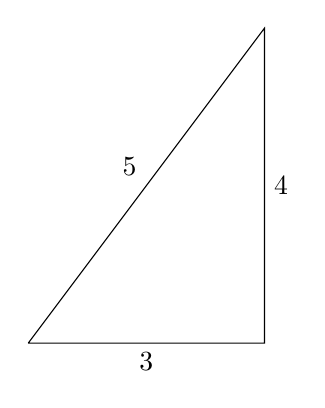
\begin{tikzpicture}
\draw[black] (0,0) -- (3,0) -- (3,4) -- (0,0);
\draw (1.5,0) node[anchor=north]{3};
\draw (3,2) node[anchor=west]{4};
\draw (1.5,2) node[anchor=south east]{5};
\end{tikzpicture}
\end{center}

If \((a,b,c)\) is a positive integer solution to the equation
\begin{equation}
a^2 + b^2 = c^2
\end{equation}
then \((a,b,c)\) is a Pythagorean triple. If \(a\), \(b\), and \(c\) have no common divisors greater than 1, then \((a,b,c)\) is a primitive (or reduced) Pythagorean triple (PPT). Similarly, if \(a^2 + b^2 = c^2\) where \((a,b,c)\) is a PPT then  \(a^2 + b^2 = c^2\) is primitive. In the following list only the second triangle is not primitive.

\begin{enumerate}
\item \(3^2 + 4^2 = 5^2\)
\item \(6^2 + 8^2 = 10^2\)
\item \(5^2 + 12^2 = 13^2\)
\item \(7^2 + 24^2 = (5^2)^2\)
\item \((15^2)^2 + 272^2 = 353^2\)
\end{enumerate}

Clearly, if \(k\) divides any two of \(a\), \(b\), and \(c\), it divides all three. And if  \(a^2 + b^2 = c^2\) then \(k^2a^2 + k^2b^2 = k^2c^2\). That is, for a positive integer \(k\), if \((a,b,c)\) is a Pythagorean triple, then so is \((ka,kb,kc)\). Hence, to find all Pythagorean triples, it's sufficient to find all primitive Pythagorean triples.

\subsection{Euclid's Formula}
\label{sec:Euclid}

Let \(a\), \(b\), and \(c\) be relatively prime positive integers such that \(a + b = c\). Set \[ \frac{m}{n} = \frac{c + a}{b} \] reduced to lowest terms; that is, \(\gcd(m,n) = 1\). From the triangle inequality \(m > n\). Then

\begin{equation}
\frac{m}{n}b - a = c.
\label{eq:a}
\end{equation}

Squaring both sides of (\ref{eq:a}) and multiplying through by \(n^2\) we get \[ m^2b^2 - 2mnab + n^2a^2 = n^2a^2 + n^2b^2,\] which, after canceling and rearranging terms, becomes

\begin{equation}
b(m^2 - n^2) = a(2mn).
\end{equation}

There are two cases, either \(m\) and \(n\) are of opposite parity, or they or both odd. Since \(\gcd(m,n)=1\), they can not both be even.

\begin{case}
\(m\) and \(n\) of opposite parity, ie. \(m\not\equiv \pm n \pmod{2}\). So 2 divides \(b\) since \(m^2 - n^2\) is odd. From equation (\ref{eq:a}), \(n\) divides \(b\). Since \(\gcd(m,n) = 1\) then \(\gcd(m, m^2 - n^2) = 1\), therefore \(m\) also divides \(b\). And since \(\gcd(a, b) = 1\), \(b\) divides \(2mn\). Therefore \(b = 2mn\). Then

\begin{equation}
\begin{aligned}
a &= m^2 - n^2, \\
b &= 2mn, \\
\text{and from (\ref{eq:a}), } c &= \frac{m}{n}2mn - (m^2 - n^2) = m^2 + n^2.
\end{aligned}
\label{eq:EuclidCase1}
\end{equation}
\end{case}

\begin{case}
\(m\) and \(n\) both odd, ie. \(m\equiv \pm n \pmod{2}\). So 2 divides \(m^2 - n^2\). Then by the same process as in the first case we have

\begin{equation}
\begin{aligned}
a &= \frac{m^2 - n^2}{2}, \\
b &= mn, \\
\text{and } c &= \frac{m^2 + n^2}{2}.
\end{aligned}
\label{eq:EuclidCase2}
\end{equation}
\end{case}

The parametric equations in (\ref{eq:EuclidCase1}) and (\ref{eq:EuclidCase2}) appear to be different but they generate the same solutions. To show this, let \[u = \frac{m + n}{2} \text{ and } v = \frac{m - n}{2}.\]

Substituting those values for \(m\) and \(n\) into (\ref{eq:EuclidCase2}) we get
\begin{equation}
\begin{aligned}
a &= 2uv, \\
b &= u^2 - v^2, \\
\text{and } c &= u^2 + v^2
\end{aligned}
\label{eq:EuclidEquiv}
\end{equation}
where \(u > v\), \(\gcd(u, v) = 1\), and \(u\) and \(v\) are of opposite parity. Therefore (\ref{eq:EuclidEquiv}), with the labels for \(a\) and \(b\) interchanged, is identical to (\ref{eq:EuclidCase1}). Thus since \(\left\{m^2-n^2, 2mn, m^2+n^2\right\}\), as in (\ref{eq:EuclidCase1}), is a primitive Pythagorean triple, we can say that \((a,b,c)\) is a primitive pythagorean triple if and only if there exists relatively prime, positive integers \(m\) and \(n\), where \(m > n\), such that \(a = m^2-n^2\), \(b=2mn\), and \(c = m^2+n^2\). And \((a,b,c)\) is a Pythagorean triple if and only if
\[ a = k(m^2 - n^2), \quad b = k(2mn), \quad\text{and } c = k(m^2 + n^2), \]
where \(k\) is a positive integer.

Alternatively, \((a,b,c)\) is a Pythagorean triple if and only if there exists relatively prime, positive integers \(u\) and \(v\), where \(u > v\), \(u \equiv v \pmod{2}\) such that \[a = k\left(\frac{u^2 - v^2}{2}\right), \quad b = k(uv), \quad\text{and } c = k\left(\frac{u^2 + v^2}{2}\right).\]

\subsection{Using Gaussian Integers}
\label{sec:PTGaussian}

Let
\begin{equation}
a^2 + b^2 = c^2
\label{eq:pythag}
\end{equation}
where \(a\), \(b\), and \(c\) are pairwise, relatively prime, positive integers. Let \(z=a+bi\) and  \(\bar{z}=a-bi\), where \(i=\sqrt{-1}\). Then \(z\) and \(\bar{z}\) are Gaussian integers, and \(\bar{z}\) is the conjugate of \(z\). Note that

\begin{equation}
\begin{aligned}
a &= \frac{z + \bar{z}}{2}, \\
b &= \frac{z - \bar{z}}{2i}, \\
\text{and } c &= \sqrt{z \bar{z}}.
\end{aligned}
\label{eq:GaussianIntegers}
\end{equation}

Since  \(\gcd(a,b)=1\), then  \(\gcd(z,\bar{z})=1\). Hence each of \(z\) and \(\bar{z}\) is a square. That is, there exists integers \(m\) and \(n\) such that  \((m+ni)^2 = z\) and  \((m-ni)^2 = \bar{z}\). So, from equation (\ref{eq:GaussianIntegers}), \[\begin{aligned} a &= \frac{(m+ni)^2 + (m-ni)^2}{2} = m^2-n^2, \\ b &= \frac{(m+ni)^2 - (m-ni)^2}{2i} = 2mn, \\ \text{and } c &= \sqrt{(m+ni)^2(m-ni)^2} = m^2+n^2. \end{aligned}\]

Since \(a\) is a positive integer, \(m\) and \(n\) must be positive integers, where \(m > n\). And since  \(\gcd(a,b) = 1\), \(m\) and \(n\) must be relatively prime and of opposite parity.

Equation (\ref{eq:GaussianIntegers}) illustrates a method for finding primitive Pythagorean triangles where the hypotenuse is to a power. We have the identity

\begin{equation}
\left\lvert \frac{z^{2k} + \bar{z}^{2k}}{2} \right\rvert^2 + \left\lvert \frac{z^{2k} - \bar{z}^{2k}}{2i} \right\rvert^2 = z^{2k}\,\bar{z}^{2k} .
\label{eq:GaussianIdentity}
\end{equation}

The absolute values are necessary since the terms on the left, depending on \(k\), which may or may not be positive.

\begin{example}
Let \(a = 3\), \(b = 4\), and \(k = 3\). Then, from equation (\ref{eq:GaussianIdentity}), we have \[ \begin{aligned} &\phantom{=\,\,} \left\lvert \frac{(3+4i)^6+(3-4i)^6}{2} \right\rvert^2 + \left\lvert \frac{(3+4i)^6-(3-4i)^6}{2i} \right\rvert^2 = (3+4i)^6 (3-4i)^6 \\ &= 11753^2 + 10296^2 = (25^3)^2. \end{aligned} \]
\end{example}

\subsection{The Difference Method}
\label{sec:PTDiff}

Let \((a,b,c)\) be a primitive Pythagorean triple. Without loss of generality, let \(a\) be odd. Equation (\ref{eq:pythag}) can be written as \[ a^2 = c^2 - b^2. \]

Set \(w = c + b\) and \(\bar{w} = c - b\). Thus

\begin{equation}
\begin{aligned}
a &= \sqrt{w \bar{w}}, \\
b &= \frac{w + \bar{w}}{2}, \\
\text{and } c &= \frac{w - \bar{w}}{2}.
\end{aligned}
\label{eq:DifferenceMethod}
\end{equation}

Since \((a,b,c)\) is primitive,  \(\gcd(c,b) = \gcd(w,\bar{w}) = 1\). This implies that each of \(w\) and \(\bar{w}\) is a square. So, since any odd positive integer greater than 1 can be written as the difference of two positive integer squares, there exists positive integers \(m\) and \(n\), where \(m > n\), such that \((m+n)^2 = w\) and \((m-n)^2 = \bar{w}\). Hence, from equation (\ref{eq:DifferenceMethod}), \[\begin{aligned} a &= \sqrt{(m+n)^2(m-n)^2} = m^2-n^2, \\ c &= \frac{(m+n)^2 + (m-n)^2}{2} = m^2+n^2, \\ \text{and } b &= \frac{(m+n)^2 - (m-n)^2}{2i} = 2mn. \end{aligned}\]

Since  \(\gcd(a,b)=1\), \(m\) and \(n\) must be relatively prime and of opposite parity.

Equation (\ref{eq:DifferenceMethod}) illustrates an efficient method for finding primitive Pythagorean triples where the odd leg is to a power. We have the identity,

\begin{equation}
w^{2k}\,\bar{w}^{2k} = \left( \frac{w^{2k} + \bar{w}^{2k}}{2} \right)^2 - \left( \frac{w^{2k} - \bar{w}^{2k}}{2} \right)^2 .
\label{eq:DifferenceIdentity}
\end{equation}

\begin{example}
Let \(c = 5\), \(b = 4\), and \(k = 3\). Then, from equation (\ref{eq:DifferenceIdentity}), we have \[ \begin{aligned} (5+4)^6 (5-4)^6 &= \left( \frac{(5+4)^6+(5-4)^6}{2} \right)^2 - \left( \frac{(5+4)^6-(5-4)^6}{2} \right)^2. \\ \text{That is, } 9^6 &= 265721^2 - 265720^2. \end{aligned} \]
\end{example}

\section{Finding \(m\) and \(n\) if given a primitive Pythagorean triple}
\label{sec:PPTmn}

\begin{quote}
\textsf{Have you ever been, while attending a rap concert, political gathering, or pro-wrestling event, asked to find numerical values for the parameters used to generate a particular primitive Pythagorean triple? And did you suffer embarrassment and scorn because you did not know how to perform such a simple task? If you answered yes to those two questions then this section is for you.}
\end{quote}

\noindent{\scshape Addendum.} \textit{Apparently, although I was unaware of this fact until recently, Jekuthiel Ginsburg was first to publish the method of finding the generating parameters for a given PPT by setting \(c+a\) (reduced to lowest terms) equal to \(m/n\), see citation} \cite[p.~188]{jg}

\begin{claim}
If \(a^2 + b^2 = c^2\) is a primitive Pythagorean triangle, where \(a\) is odd, then each of the fractions \[ \frac{c+a}{b}, \quad \frac{c+b+a}{c+b-a}, \quad
\frac{b}{c-a}, \quad \text{and } \frac{a+c-b}{a+b-c} \] (each fraction reduced to lowest terms) is equal to \(m/n\), where \[ a = m^2-n^2, \quad b = 2mn, \quad \text{and } c = m^2+n^2. \]
\end{claim}

\begin{proof}
\begin{align*}
\frac{c+a}{b} &= \frac{\left(m^2+n^2\right)+\left(m^2-n^2\right)}{2mn} &= \frac{2m^2}{2mn} &= \frac{m}{n}, \\
\frac{c+b+a}{c+b-a} &= \frac{\left(m^2+n^2\right)+(2mn)+\left(m^2-n^2\right)} {\left(m^2+n^2\right)+(2mn) - \left(m^2-n^2\right)} &= \frac{2m(m+n)}{2n(n+m)}&= \frac{m}{n}, \\
\frac{b}{c-a} &= \frac{2mn}{\left(m^2+n^2\right)-\left(m^2-n^2\right)} &= \frac{2mn}{2n^2} &= \frac{m}{n}, \\
\text{and} \quad \frac{a+c-b}{a+b-c} &=\frac{\left(m^2-n^2\right)+\left(m^2+n^2\right)-(2mn)}{\left(m^2-n^2\right)+(2mn)-\left(m^2+n^2\right)} &= \frac{2m(m-n)}{2n(m-n)} &= \frac{m}{n}.
\end{align*}
\end{proof}

\begin{claim}
If \(a^2 + b^2 = c^2\) is a primitive Pythagorean triangle, where \(a\) is even, then each of the fractions \[ \frac{c+a}{b}, \quad \frac{c+b+a}{c+b-a}, \quad
\frac{b}{c-a}, \quad \text{and } \frac{a+c-b}{a+b-c} \] (each fraction reduced to lowest terms) is equal to \(m/n\), where \[ a = \frac{m^2-n^2}{2}, \quad b = mn, \quad \text{and } c = \frac{m^2+n^2}{2}. \]
\end{claim}

\begin{proof}
Since \((a,b,c)\) is a PPT, there exists relatively prime, positive integers, \(u\) and \(v\), where \(u > v\), and \(u\) is of opposite parity to \(v\) such that \[ a = 2uv, \qquad b = u^2 - v^2, \quad\text{and } c = u^2 + v^2. \]

So,

\begin{align*}
\frac{c+a}{b} &= \frac{u^2+v^2+2uv}{u^2-v^2} &= \frac{(u+v)^2}{(u+v)(u-v)} &= \frac{u+v}{u-v}, \\
\frac{c+b+a}{c+b-a} &=  \frac{u^2+v^2+u^2-v^2+2uv}{u^2+v^2+u^2-v^2-2uv} &= \frac{2u(u+v)}{2u(u-v)}&= \frac{u+v}{u-v}, \\
\frac{b}{c-a} &= \frac{u^2-v^2}{u^2+v^2-2uv} &= \frac{(u+v)(u-v)}{(u-v)^2} &= \frac{u+v}{u-v}, \\
\frac{a+c-b}{a+b-c} &=  \frac{2uv+u^2+v^2-u^2+v^2}{2uv+u^2-v^2-u^2-v^2} &= \frac{2v(u+v)}{2v(u-v)}  &= \frac{u+v}{u-v}.
\end{align*}

Let \(m = u + v\) and \(n = u - v\). Then \[u = \frac{m + n}{2} \text{ and } v = \frac{m - n}{2}.\]

Hence, we have \[ a = 2uv = \frac{m^2-n^2}{2}, \quad b = u^2-v^2 = mn, \quad \text{and } c = u^2+v^2 = \frac{m^2+n^2}{2}. \]

\end{proof}

\begin{example}
\( 3^2 + 4^2 = 5^2 \) is a PPT and 3 is \underline{odd}. So, let \(a = 3\). Then \[ \frac{5+3}{4} = \frac{5+4+3}{5+4-3} = \frac{4}{5-3} = \frac{3+5-4}{3+4-5} = \frac{2}{1}.\]

Hence \[ 3=2^2-1^2, \quad 4=2(2)(1), \quad \text{and } 5=2^2+1^2. \]

\noindent Alternatively, \(4^2 + 3^2 = 5^2\) is a PPT and 4 is \underline{even}. So, let \(a = 4\). Then \[ \frac{5+4}{3} = \frac{5+3+4}{5+3-4} = \frac{3}{5-4} = \frac{4+5-3}{4+3-5} = \frac{3}{1}. \]

Hence \[ 4=\frac{3^2-1^2}{2}, \quad 3=(3)(1), \quad \text{and } 5=\frac{3^2+1^2}{2}. \]
\end{example}

\begin{example}
\( 21^2 + 20^2 = 29^2 \) is a PPT and 21 is \underline{odd}. So, let \(a = 21\). Then \[ \frac{29+21}{20} = \frac{29+20+21}{29+20-21} = \frac{20}{29-21} = \frac{21+29-20}{21+20-29} = \frac{5}{2}. \]

Hence \[ 20=2(5)(2), \quad 21=5^2-2^2, \quad \text{and }
29=5^2+2^2. \]

\noindent Alternatively, \(20^2 + 21^2 = 29^2\) is a PPT and 20 is \underline{even}. So, let \(a = 20\). Then \[ \frac{29+20}{21} = \frac{29+21+20}{29+21-20} = \frac{21}{29-20} = \frac{20+29-21}{20+21-29} = \frac{7}{3}. \]

Hence \[ 20 = \frac{7^2-3^2}{2}, \quad 21=(7)(3), \quad \text{and } 29 = \frac{7^2+3^2}{2}. \]
\end{example}

\section{Pythagorean triples and the divisors 3, 4, and 5}

\begin{claim}
If \((a,b,c)\) is a solution in positive integers to the equation  \(a^2+b^2 = c^2\) then 3 divides \(a\) or \(b\), 4 divides \(a\) or \(b\), and 5 divides \(a\), \(b\), or \(c\).
\end{claim}

\begin{proof}
\begin{case} (The divisor 3) Every integer squared equals 0 or 1 modulo 3. Hence, if \(3\nmid ab\) then \(a^2+b^2 = c^2 = 1+1 = 2\) modulo 3. But \(c^2= 0\) or 1 modulo 3. Therefore \(3 \mid ab\).
\end{case}
\begin{case} (The divisor 4) Every square integer equals 0, 1, 4, or 9 modulo 16. If \(4\nmid b\) then \(b^2\) equals either of 1, 4, or 9 modulo 16. But none of  \(1+1, 1+4, 1+9, 4+4, 4+9\), or \(9+9\) equals 0, 1, 4, or 9 modulo 16. However, \(c^2\) equals 0, 1, 4 or 9 modulo 16. Hence \(a^2\) must equal 0 modulo 16. That is, 16 divides \(a^2\) and 4 divides \(a\).
\end{case}
\begin{case} (The divisor 5) Every integer squared equals 0, 1, or 4 modulo 5. If \(5\nmid ab\) then \(a^2 + b^2 = 1+1\), 1+4, or 4+4, which equals 2, 0, or 3 modulo 5. But \(c^2\) equals 0, 1, or 4 modulo 5. Therefore  \(a^2 + b^2 = c^2 = 0\) modulo 5 implies \( 5\mid c \).
\end{case}
\end{proof}

Later, in section 5.1 ``Some prime divisors of primitive Pythagorean triangles" the following generalizations are found for the divisors 3, 4, and 5.

Let \(a^2 + b^2 = (c^k)^2\) where \(k \in \mathbb{Z}^+\). Let \(d\) be a positive integer divisor of \(k\).

\begin{enumerate}
\item If \(p=4d-1\) is a prime then \(p\) divides either \(a\) or \(b\).
\item If \(d=2^j\), where \(j\) is a non-negative integer, then  \(2^{j+2}\) divides either \(a\) or \(b\).
\item If \(q=4d+1\) is a prime then \(q\) divides one of \(a\), \(b\), or \(c\).
\end{enumerate}

Set \(d=1\), then \(p=4(1)-1=3\), \(d=2^j=1\) implies \(j=0\) implies \(2^{0+2}=4\), and \(q=4(1)+1=5\).

\section{Primitive Pythagorean triangles where \(a - b\) is a constant}

Finding primitive Pythagorean triangles with a given difference between the lengths of the hypotenuse and a leg is a simple matter; from the parametrization (\ref{eq:EuclidCase1}), \[ a = m^2 - n^2, \quad b = 2mn, \quad\text{and } c = m^2 + n^2, \] \(c-a=2n^2\) and \(c-b=(m-n)^2\). So, just choose the proper \(m\) and/or \(n\).

However, finding Pythagorean triangles with constant difference between the lengths of the two smaller legs leads to a \textbf{Pell Equation} \[ a-b = m^2-n^2-2mn = (m-n)^2-2n^2 = d. \]

Hence, if one solution is found, other solutions can be found recursively, from which a closed form can be obtained.

The following scheme does not find solutions for every integer \(d\), only those where \(d=\pm (2t^2-1)\), and not all of those. For example, in the Pythagorean triangle  \(35^2+12^2 = 37^2\), there exists no integer \(t\) such that \(2t^2-1=23\), and the scheme does not generate the triangle \(15^2+8^2 = 17^2\) where \(2 (2)^2-1=7\).

I'll use the alternative parametrization from equation (\ref{eq:EuclidCase2}): \((a,b,c)\) is a primitive Pythagorean triple if and only if there exists relatively prime, odd positive integers \(m\) and \(n\), where \(m > n\), such that \[ a = mn, \quad b = \frac{m^2-n^2}{2},\quad\text{and } c = \frac{m^2+n^2}{2}.\]

I'll give a closed form for \(a\) and \(b\) where  \(a-b = \pm
(2t^2-1)\). Let

\begin{equation}
f(s) = \frac{(1+\sqrt{2})^s + (1-\sqrt{2})^s}{2},
\end{equation}
and
\begin{equation}
g(s) = t\, f(s) - (t-1)\, f(s-1),
\end{equation}
where \(s\) and \(t\) are positive integers. Set

\begin{equation}
\begin{aligned}
a &= g(s+1)\, g(s), \\
b &= \frac{g(s+1)^2 - g(s)^2}{2}, \\
\text{and } c &= \frac{g(s+1)^2 + g(s)^2}{2}.
\end{aligned}
\label{eq:ABConstant}
\end{equation}

\begin{claim}
For positive integers \(s\) and \(t\) where \((a,b,c)\) is as defined in (\ref{eq:ABConstant}),
\begin{enumerate}
\item \(2f(s) + f(s-1) = f(s+1)\),
\item \(2g(s) + g(s-1) = g(s+1)\),
\item \(\gcd(g(s), g(s+1)) = 1\),
\item \((a,b,c)\) is a primitive Pythagorean triple, and
\item \(a-b = (-1)^s (2t^2 - 1)\).
\end{enumerate}
\end{claim}

\begin{proof}
\begin{case}
\[\begin{aligned} 2 f(s)+f(s-1) &= \frac{(1+\sqrt{2})^{s-1} \big(2(1+\sqrt{2})\big) + (1-\sqrt{2})^{s-1} \big(2(1-\sqrt{2})+1\big)}{2} \\   
&= \frac{(1+\sqrt{2})^{s-1} (1+\sqrt{2})^2 + (1-\sqrt{2})^{s-1} (1-\sqrt{2})^2}{2} \\
&= \frac{(1+\sqrt{2})^{s+1} + (1-\sqrt{2})^{s+1}}{2} \\ &= f(s+1). \end{aligned} \]
\end{case}
\begin{case}
\[\begin{aligned}
2 g(s)+g(s-1) &= 2\big(t f(s)-(t-1) f(s-1)\big) + \big(t f(s-1)-(t-1) g(f-2)\big) \\ &= t\big(2 f(s)+f(s-1)\big)-(t-1)\big(2 f(s-1)+f(s-2)\big) \\ &= t f(s+1)-(t-1) f(s) \hskip0.27\textwidth \text{from case 1} \\ &= g(s+1).
\end{aligned}\]
\end{case}
\begin{case}
\(d\mid g(s+1)\) and \(d\mid g(s)\) implies  \(d\mid g(s+1)-2 g(s)=g(s-1)\), from case 2. Then \(d\vert g(s)\) and \(d\mid g(s-1)\) implies  \(d\mid g(s-2)\). And so on, until ultimately, \(d\mid g(0)=-1\).
\end{case}
\begin{case}
\(g(s+1)\) and \(g(s)\) are relatively prime, odd, positive integers, such that \(g(s+1)>g(s)\) where \(a^2+b^2=c^2\).
\end{case}
\begin{case}
If \(s=1\), then
\[\begin{aligned}
f(s+1) &= f(2) &=3, \\
f(s) &= f(1) &=1, \\
f(s-1) &= f(0) &=1.
\end{aligned}\]

Thus
\[\begin{aligned}
a &= g(s+1) = t f(2)-(t-1) f(1) = 3t-(t-1) = 2t+1. \\
b &= g(s)= t f(1)-(t-1) f(0) = t-(t-1) = 1.
\end{aligned}\]

Then, from (\ref{eq:ABConstant}), \[ a-b = (2t+1)(1) -\left( \frac{(2t+1)^2-1^2}{2} \right) = (-1)^1 \left(2t^2-1\right).
\]

So the claim is true for \(s = 1\). By induction on \(s\), assume it's true for \(s = r\). That is, assume \[ a-b = \frac{2 g(r+1) g(r)-g(r+1)^2+g(r)^2}{2} = (-1)^r(2t^2-1). \]

Then, for \(s = r+1\),
\[ \begin{aligned}
a - b &=\frac{2 g(r+2) g(r+1)-g(r+2)^2+g(r+1)^2}{2} \\
&= \frac{g(r+2)\big((2 g(r+1)-g(r+2)\big)+g(r+1)^2}{2} \\
&= \frac{\big(2 g(r+1)+g(r)\big)(-g(r))+g(r+1)^2}{2} \\
&= \frac{-2 g(r+1) g(r)-g(r)^2+g(r+1)^2}{2} \\
&=-\left(\frac{2 g(r+1) g(r)-g(r+1)^2+g(r)^2}{2}\right) \\
&=-(-1)^r(2t^2-1) = (-1)^{r+1}(2t^2-1).
\end{aligned} \]
\end{case}
\end{proof}

\begin{example}
\( a - b = \pm 1\).

\smallskip

\begin{minipage}{0.9\textwidth}
\centering
\begin{tabular}{rr|rr|rrr}
\(t\) & \(s\) & \(g(s+1)\) & \(g(s)\) & \(a\) & \(b\) & \(c\) \\ \hline
1 & 1 & 3 & 1 &   3 &  4 &  5 \\
1 & 2 & 7 & 3 &  21 & 20 & 29 \\
1 & 3 &17 & 7 & 119 &120 &169 \\
1 & 4 &41 &17 & 697 &696 &985 \\
1 & 5 &99 &41 &4059&4060&5741
\end{tabular}
\end{minipage}
\label{tab:example}
\end{example}

\begin{example}
\( a - b = \pm 7\).

\smallskip

\begin{minipage}{0.9\textwidth}
\centering
\begin{tabular}{rr|rr|rrr}
\(t\) & \(s\) & \(g(s+1)\) & \(g(s)\) & \(a\) & \(b\) & \(c\) \\ \hline
2 & 1 & 5 & 1 &   5 & 12 & 13 \\
2 & 2 &11 & 5 &  55 & 48 & 73 \\
2 & 3 &27 &11 & 297 &304 &425 \\
2 & 4 &65 &27 &1755&1748&2477 \\
2 & 5 &157&65 &10205&10212&14437
\end{tabular}
\end{minipage}
\end{example}

\begin{example}
\( a - b = \pm 97\).

\smallskip

\begin{minipage}{0.9\textwidth}
\centering
\begin{tabular}{rr|rr|rrr}
\(t\) & \(s\) & \(g(s+1)\) & \(g(s)\) & \(a\) & \(b\) & \(c\) \\ \hline
7 & 1 &15 & 1 &  15 &112 &113 \\
7 & 2 &31 &15 & 465 &368 &593 \\
7 & 3 &77 &31 &2387&2484&3445 \\
7 & 4 &185&77 &14245&14148&20077 \\
7 & 5 &447&185&82695&82792&117017
\end{tabular}
\end{minipage}
\end{example}

\subsection{Pythagorean triple preserving matrices}

From example \ref{tab:example}, let \[\mathbf{C} = \begin{pmatrix} 3 & 4 & 5 \\ 21 & 20 & 29 \\ 119 & 120 & 169 \end{pmatrix} \quad\text{and}\quad \mathbf{D} = \begin{pmatrix} 21 & 20 & 29 \\ 119 & 120 & 169 \\ 697 & 696 & 985 \end{pmatrix}.\]

So, solving for \(\mathbf{A}\) in the matrix equation \(\mathbf{C}\mathbf{A}=\mathbf{D}\), we find that \[\mathbf{A} = \begin{pmatrix}1 & 2 & 2 \\ 2 & 1 & 2 \\ 2 & 2 & 3 \end{pmatrix}.\]

Let \(a^2+b^2=c^2\). Then \( \begin{pmatrix}a&b&c\end{pmatrix}\mathbf{A}=\begin{pmatrix}u&v&w\end{pmatrix}\) where \(u^2+v^2=w^2\), and \(u-v=b-a\). Furthermore,\[ \begin{pmatrix}
m^2-n^2&2mn&m^2+n^2
\end{pmatrix}\begin{pmatrix} 1 & 2 & 2 \\ 2 & 1 & 2 \\ 2 & 2 & 3 \end{pmatrix}= \begin{pmatrix} \mu^2-\nu^2 & 2\mu\nu & \mu^2+\nu^2 \end{pmatrix} \] where \(\mu=2m+n\) and \(\nu=m\). Therefore, if \((a,b,c)\) is a primitive Pythagorean triple then so is \((u,v,w)\). Thus, if  \(n\in
\mathbb{Z}^+ \), then \(\begin{pmatrix}1 & 0 & 1\end{pmatrix}\mathbf{A}^n = \begin{pmatrix}u_n & v_n & w_n\end{pmatrix}\) gives the \(n^{\mathrm{th}}\) primitive Pythagorean triple such that \(u_n-v_n=\pm 1\).

\subsection{\(c-a\) or \(c-b\) a constant by matrix action}

We have, using matrix \(\mathbf{A}\), if \((a,b,c)\) is a primitive Pythagorean triple then \[ \begin{pmatrix} -a&b&c \end{pmatrix} \begin{pmatrix} 1&2&2 \\ 2&1&2 \\ 2&2&3 \end{pmatrix} = \begin{pmatrix} a&b&c \end{pmatrix} \begin{pmatrix} -1&-2&-2 \\ 2&1&2 \\ 2&2&3 \end{pmatrix} = \begin{pmatrix}r&s&t \end{pmatrix} \] where \(r\), \(s\), and \(t\) are pairwise relatively prime, \( r^2+s^2 = t^2\), and \[ t-r = (-2a+2b+3c)-(-a+2b+2c) = c-a.\]

Also, \(r\), \(s\), and \(t\) are positive integers, since \(c>a\). Hence \((r,s,t)\) is a primitive Pythagorean triple.

Similarly, if \((a,b,c)\) is a primitive Pythagorean triple then \[ \begin{pmatrix} a&b&c \end{pmatrix} \begin{pmatrix} 1&2&2 \\ -2&-1&-2 \\ 2&2&3 \end{pmatrix} = \begin{pmatrix}x&y&z \end{pmatrix} \] where \((x,y,z)\) is a primitive Pythagorean triple such that \(z-y = c-b\).

Let \[ \mathbf{D} = \begin{pmatrix} -1&-2&-2 \\ 2&1&2 \\ 2&2&3 \end{pmatrix} \quad\text{and}\quad \mathbf{U} = \begin{pmatrix} 1&2&2 \\ -2&-1&-2 \\ 2&2&3 \end{pmatrix}. \]

Joe Roberts\textsuperscript{\cite{jr}} has shown that \((a, b, c)\) is a primitive Pythagorean triple if and only if \[ \begin{pmatrix} a & b & c \end{pmatrix} = \begin{pmatrix} 3 & 4 & 5 \end{pmatrix} \mathfrak{R} \] where \(\mathfrak{R}\) is a finite product of the matrices \(\textbf{U}\), \(\textbf{A}\), and \(\textbf{D}\).

\section{Primitive Pythagorean triangles where the hypotenuse is to a power}

\begin{quote}
\textsf{It is well-known that if \((a,b,c)\) is a solution to a Pythagorean triangle, where \(c\) is the hypotenuse, then the Mersenne prime \(3\) divides \(ab\), and the Fermat prime \(5\) divides \(abc\). In this section, I show that if \((a,b,c^{2^j})\) is a solution to a primitive Pythagorean triangle, where \(j\) is a non-negative integer, then every Mersenne prime less than or equal to \((2^{j+2}-1)\) divides \(ab\), and every Fermat prime less than or equal to \((2^{j+2}+1)\) divides \(abc\).}
\end{quote}

All PPTs are given by the parametric equations
\begin{equation}
\begin{aligned}
a &= m^2 - n^2, \\
b &= 2mn, \\
\text{and } c &= m^2 + n^2
\end{aligned}
\end{equation}
where \(m\) and \(n\) are relatively prime, positive integers of opposite parity, and \(m > n\).

When computing the PPT \((a,b,c^{2^j})\), it is convenient to express \(a\), \(b\), and \(c\) in terms of Gaussian integers \(\mathbb{Z}[i]\). To do so, let \(m > n\) where \(m\) and \(n\) are relatively prime, positive integers having opposite parity. Let \(z=m+ni\),  \(\bar{z}=m-ni\), and \(j\) be a non-negative integer. Then there exists positive integers \(u\) and \(v\) such that \[\begin{aligned} u &= \left\lvert \frac{z^{2^j}+\bar{z}^{2^j}}{2} \right\rvert = \left\lvert\frac{(u+vi)+(u-vi)}{2}\right\rvert, \\ \text{and } v &= \left\lvert\frac{z^{2^j}-\bar{z}^{2^j}}{2i}\right\rvert = \left\lvert\frac{(u+vi)-(u-vi)}{2i}\right\rvert. \end{aligned}\]

\begin{itemize}
\item If \(u < v\) then interchange the labels.
\item Clearly, \(\gcd(m,n)=1\) implies \(\gcd(u,v)=1\).
\item The parameters \(m\) and \(n\) have opposite parity. Therefore \( 2\nmid (m^2+n^2)^{2^j} = u^2+v^2\). Hence \(u\) and \(v\) have opposite parity.
\end{itemize}

Thus, all primitive Pythagorean triples of the form  \((a,b,c^{2^j})\) are given by the parametric equations

\begin{align}
a &= u^2-v^2 &= \left\lvert \frac{(m+ni)^{2^{j+1}}+(m-ni)^{2^{j+1}}}{2} \right\rvert, \\
b &= 2uv &= \left\lvert \frac{(m+ni)^{2^{j+1}}-(m-ni)^{2^{j+1}}}{2i} \right\rvert, \\
\text{and } c^{2^j} &= u^2+v^2 &= (m^2+n^2)^{2^j}.
\end{align}

Then
\begin{equation}
2ab = \left\lvert \frac{(m+ni)^{2^{j+2}}-(m-ni)^{2^{j+2}}}{2i} \right\rvert.
\label{eq:hypotenuse}
\end{equation}

\subsection{Some prime divisors of primitive Pythagorean triangles}

If \(a\), \(b\), \(c\), \(k\) and \(d\) are positive integers such that \( a^2+b^2 = (c^k)^2\) is a primitive Pythagorean triangle, and if \(d\) divides \(k\), then we are going to show the following:

\begin{itemize}
\item If \(4d-1\) is a prime \(p\), then \(p\) divides exactly one of \(a\) and \(b\).
\item If \(4d+1\) is a prime \(q\), then \(q\) divides exactly one of \(a\), \(b\), and \(c\).
\item If \(d=2^{\alpha}\), where \(\alpha\) is a non-negative integer, then \(2^{\alpha+2}\) divides exactly one of \(a\) and \(b\).
\end{itemize}

Previously, it was shown in section 3, that those three items are true for the case \(d=1\).

I will, first, state and prove a theorem on the divisors of \(ab\), and of \(abc\), where \((a,b,c^k)\) is a PPT. Then the case where \(k=2^j\) will be proven in the corollary. If \(k=2^j\) in equation (\ref{eq:hypotenuse}) then \[2ab = \left\lvert \frac{(m+ni)^{4k}-(m-ni)^{4k}}{2i} \right\rvert.\]

\begin{theorem}
Let \(a^2+b^2 = (c^k)^2\) be a primitive Pythagorean triangle where \(k\in \mathbb{Z}^+\). Let \(d\) be a positive integer divisor of \(k\). Let  \(p = 4d-1\) and \(q = 4d+1\).
\label{th:Prime}
\end{theorem}
\renewcommand{\labelenumi}{(\alph{enumi})}
\begin{enumerate}
\item If \(p\) is prime then \(p\mid ab\).
\item If \(q\) is prime then \(q\mid abc\).
\end{enumerate}
\begin{proof}
\begin{case}
Since \(m+ni \in \mathbb{Z}[i]\), then  \(((m+ni)^{k/d})^{4d} = (M+Ni)^{4d}\) for some  \(M, N\in \mathbb{Z}\). If \(p=4d-1\) is a prime, then since \(-i=i^{4d-1}=i^p\), \[ p \mid (M+Ni)^p-(M-Ni)= [ (M+Ni)^p - M^p - (Ni)^p ] + (M^p-M)-i(N^p-N), \] which implies \[ p\mid (M+Ni)^{p+1} - (M^2+N^2). \]

Similarly, \[ p\mid (M-Ni)^{p+1} - ( M^2+N^2 ), \] which implies \[ p \mid  (M+Ni)^{p+1}-(M-Ni)^{p+1} = (m+ni)^{4k}-(m-ni)^{4k} = 4abi. \]

Therefore \(p\mid ab\).
\end{case}
\begin{case}
If \(q = 4d+1\) is a prime, then since  \(i = i^{4d+1} = i^q\), \( q\mid(M+Ni)^q - (M+Ni)\) where  \(M+Ni=(m+ni)^{k/d}\) and \(M-Ni=(m-ni)^{k/d}\). Which implies \[ q\mid (M+Ni) \big((M+Ni)^{q-1}-1\big). \]

Similarly, \[ q\mid(M-Ni) \big((M-Ni)^{q-1}-1\big). \]

Then, if \( q\nmid (M+Ni)(M-Ni) = M^2+N^2 = c^{k/d}, \) \[ q \mid (M+Ni)^{q-1}-(M-Ni)^{q-1} = (m+ni)^{4k}-(m-ni)^{4k}=4abi. \]

Therefore \(q \mid abc\).
\end{case}
\end{proof}

\begin{corollary}
Let \(a^2+b^2 = (c^{2^j})^2\) be a primitive Pythagorean triangle where \(j\) is a nonnegative integer. Let \(M\) be any Mersenne prime less than or equal to \(2^{j+2}-1\). And let \(F\) be any Fermat prime less than or equal to \(2^{j+2}+1\). Then \(M\) divides \(ab\), \(F\) divides \(abc\). \label{th:Marsenne}
\end{corollary}

\begin{proof}
Let \(k=2^j\) in theorem (\ref{th:Prime}). Then \[\begin{aligned} d &= \left\{ 2^0, 2^1, 2^2,\ldots , 2^{j-1}, 2^j \right\}, \\ 4d-1 &=\left\{ 2^2-1, 2^3-1, 2^4-1,\ldots ,2^{j+1}-1, 2^{j+2}-1 \right\}, \\ \text{and } 4d+1 &= \left\{ 2^2+1, 2^3+1, 2^4+1,\ldots ,2^{j+1}+1, 2^{j+2}+1 \right\}.
\end{aligned}\]
From theorem (\ref{th:Prime}) case 1, every prime in the set \(4d-1\) divides \(ab\). From theorem (\ref{th:Prime}), case 2, every prime in the set \(4d+1\) divides \(abc\).
\end{proof}

\subsection{The divisor \(4 = 2^{0+2}\)}

\begin{theorem}
If \(a^2+b^2 = (c^{2^j})^2\)
is a primitive Pythagorean triangle where \(j\) is a nonnegative integer then \(2^{j+2}\) divides \(ab\).
\label{th:Divisor}
\end{theorem}
\begin{proof}
If \(j=0\) then \[ a^2+b^2 = (c^{2^0})^2 = c^2. \]

So there exists integers \(m\) and \(n\), one odd the other even, such that \(a=m^2-n^2\) and \(b=2mn\). Hence \(4=2^{0+2}\) divides \(ab\). By induction on \(j\), Assume true for any \(j+1\), then \[ (c^{2^{j+1}})^2 = \left((c^{2^j})^2\right)^2
= (a^2+b^2)^2 = (a^2-b^2)^2 + (2ab)^2. \]

Let \(a_1=a^2-b^2\) and \(b_1=2ab\). Then if \(2^{j+2}\) divides \(ab\), \(2^{(j+1)+2}\) divides \(a_1b_1\).
\end{proof}

\begin{example} Divisors of primitive Pythagorean triples (\(c\) is to a power).

\bigskip

\begin{minipage}{0.9\textwidth}
\centering
\begin{tabular}{c|cl|ll}
Triangle & \(k\) & \(d\) & Divisors of \(a\) or \(b\) & Divisors of \(a\), \(b\), or \(c\) \\[2pt] \hline
\(a^2+b^2=c^2\) & 1 & 1 & \(3, 2^2\) & \(3, 2^2, 5\) \\
\(a^2+b^2=(c^2)^2\) & 2 & 1, 2 & \(3, 7, 2^3\) & \(3, 5, 7, 2^3\) \\
\(a^2+b^2=(c^3)^2\) & 3 & 1, 3 & \(3, 2^2, 11\) & \(3, 2^2, 5, 11, 13\) \\
\(a^2+b^2=(c^4)^2\) & 4 & 1, 2, 4 & \(3, 7, 2^4\) & \(3, 5, 7, 2^4, 17\) \\
\(a^2+b^2=(c^5)^2\) & 5 & 1, 5 & \(3, 2^2, 19\) & \(3, 2^2, 5, 19\) \\
\(a^2+b^2=(c^6)^2\) & 6 & 1, 2, 3, 6 & \(3, 7, 2^3, 11, 23\) & \(3, 5, 7, 2^3, 11, 13, 23\) \\
\(a^2+b^2=(c^7)^2\) & 7 & 1, 7 & \(3, 2^2\) & \(3, 2^2, 5, 29\) \\
\(a^2+b^2=(c^8)^2\) & 8 & 1, 2, 4, 8 & \(3, 7, 31, 2^5\) & \(3, 5, 7, 17, 31, 2^5\) \\
\(a^2+b^2=(c^9)^2\) & 9 & 1, 3, 9 & \(3, 2^2, 11\) & \(3, 2^2, 5, 11, 13, 37\) \\
\(a^2+b^2=(c^{10})^2\) & 10 & 1, 2, 5, 10 & \(3, 7, 2^3, 19\) & \(3, 5, 7, 2^3, 19, 41\)
\end{tabular}
\end{minipage}
\label{tab:Hypotenuse}
\end{example}

\section{Primitive Pythagorean triples where the odd leg is to a power}

\begin{quote}
\textsf{Generalizations on the well known Pythagorean triple divisors, \(3\), \(4\), and \(5\).}
\end{quote}

Let the ordered triple \((a^k,b,c)\) be a primitive Pythagorean triple where \(k\) is a positive integer and \(a\) is the odd leg. Then there exists relatively prime odd positive integers \(m\) and \(n\) where \(m > n\) such that

\begin{equation}
\begin{aligned}
a^k &= mn, \\
b &= \frac{m^2 - n^2}{2} \\
\text{and } c &= \frac{m^2 + n^2}{2}.
\end{aligned}
\label{eq:OddLegPythag}
\end{equation}

Since \(m\) and \(n\) are relatively prime, \(m=u^k\) and \(n=v^k\) for some odd positive integers \(u\) and \(k\). Then equation (\ref{eq:OddLegPythag}) becomes

\begin{equation}
\begin{aligned}
a^k &= u^kv^k, \\
b &= \frac{u^{2k} - v^{2k}}{2} \\
\text{and } c &= \frac{u^{2k} + v^{2k}}{2}.
\end{aligned}
\label{eq:OddLegPower}
\end{equation}

\begin{theorem}
If \(a\) is odd, and \((a^k,b,c)\) is a primitive Pythagorean triple, \(k\) and \(d\) are positive integers such that \(d\) divides \(k\) then:
\end{theorem}
\begin{enumerate}
\item If \(p=2d+1\) is prime then \(p\) divides one of \(a\) or \(b\).
\item If \(q=4d+1\) is prime then \(q\) divides one of \(a\), \(b\) or \(c\).
\end{enumerate}

\begin{proof}
From equation (\ref{eq:OddLegPower}),

\begin{equation}
2ab = uv\left(u^{2k} - v^{2k}\right) \quad\text{and}\quad 4abc = uv\left(u^{4k} - v^{4k}\right).
\label{eq:OddLegProofs1}
\end{equation}

If \(d\) is a divisor of \(k\) then \(k=k_1d\) where \(k_1\) is the integer \(k/d\). Thus, we can rewrite equations (\ref{eq:OddLegProofs1}) as

\begin{equation}\begin{aligned}
2a^{k_1}b &= u^{k_1}v^{k_1} \big((u^{k_1})^{2d}-(v^{k_1})^{2d}\big) \\ \text{and } 4a^{k_1}bc &= u^{k_1}v^{k_1} \big((u^{k_1})^{4d}-(v^{k_1})^{4d}\big).
\end{aligned}
\label{eq:OddLegProofs2}
\end{equation}

(Note: If a prime \(P\) divides \(a^{k_1}\) then \(P\) divides \(a\).)

Therefore, from equation (\ref{eq:OddLegProofs2}) and \textit{Fermat's little theorem}, if prime \(p=2d+1\) then \(p\) divides \(ab\). And if prime \(q=4d+1\) then \(q\) divides \(abc\). That is, since \(a\), \(b\), and \(c\) are pairwise relatively prime, \(p=2d+1\) divides exactly one of \(a\) or \(b\) and \(q=4d+1\) divides exactly one of \(a\), \(b\), or \(c\).
\end{proof}

\begin{theorem}
If \((a^{2^j},b,c)\) is a primitive Pythagorean triple where \(j\) is a nonnegative integer and \(a\) is odd then \(2^{j+2}\) divides \(b\).
\end{theorem}

\begin{proof}
The theorem is clearly true for \(j=0\). Then, by induction on \(j\), assume it's true for \(j+1\). That is, assume if \[(a^{2^j})^2=c^2-b^2 \] then \(2^{j+2}\) divides the even side \(b\).

\[ (a^{2^{j+1}})^2 = (a^{2^j})^2 (a^{2^j})^2 = (c^2-b^2)^2 = (c^2+b^2)^2 - (2cb)^2. \]

Therefore \(2(2^{j+2}) = 2^{(j+1)+2}\) divides \(2bc\).
\end{proof}

\begin{example} Divisors of primitive Pythagorean triples (\(a\) is to a power).

\bigskip

\begin{minipage}{0.9\textwidth}
\centering
\begin{tabular}{c|cl|ll}
Triangle & \(k\) & \(d\) & Divisors of \(a\) or \(b\) & Divisors of \(a\), \(b\), or \(c\) \\[2pt] \hline
\(a^2+b^2=c^2\) & 1 & 1 & \(3, 2^2\) & \(3, 2^2, 5\) \\
\((a^2)^2+b^2=c^2\) & 2 & 1, 2 & \(3, 5, 2^3\) & \(3, 5, 2^3\) \\
\((a^3)^2+b^2=c^2\) & 3 & 1, 3 & \(3, 2^2, 7\) & \(3, 2^2, 5, 7, 13\) \\
\((a^4)^2+b^2=c^2\) & 4 & 1, 2, 4 & \(3, 5, 2^4\) & \(3, 5, 2^4, 17\) \\
\((a^5)^2+b^2=c^2\) & 5 & 1, 5 & \(3, 2^2, 11\) & \(3, 2^2, 5, 11\) \\
\((a^6)^2+b^2=c^2\) & 6 & 1, 2, 3, 6 & \(3, 5, 7, 2^3, 13\) & \(3, 5, 7, 2^3, 13\) \\
\((a^7)^2+b^2=c^2\) & 7 & 1, 7 & \(3, 2^2\) & \(3, 2^2, 5, 29\) \\
\((a^8)^2+b^2=c^2\) & 8 & 1, 2, 4, 8 & \(3, 5, 17, 2^5\) & \(3, 5, 17, 2^5\) \\
\((a^9)^2+b^2=c^2\) & 9 & 1, 3, 9 & \(3, 2^2, 7, 19\) & \(3, 2^2, 5, 7, 13, 19, 37\) \\
\((a^{10})^2+b^2=c^2\) & 10 & 1, 2, 5, 10 & \(3, 5, 2^3, 11\) & \(3, 5, 2^3, 11, 41\)
\end{tabular}
\end{minipage}
\end{example}

\section{Area of a primitive Pythagorean triangle and the perfect numbers}

A perfect number is a positive integer that is equal to the sum of its divisors excluding itself. For example \(6\) is a perfect number since its divisors are \(1\), \(2\), \(3\) and \(6\), where \(1+2+3=6\). All even perfect numbers are of the form \(2^{s-1} (2^s-1)\) where \(2^s-1\) is a prime. Such primes are called Mersenne primes. The first five perfect numbers are

\renewcommand{\labelenumi}{\arabic{enumi}.}
\begin{enumerate}
\item \(2^1 (2^2 - 1) = 6\),
\item \(2^2 (2^3 - 1) = 28\),
\item \(2^4 (2^5 - 1) = 496\),
\item \(2^6 (2^7 - 1) = 8128\),
\item \(2^{12} (2^{13} - 1) = 33550336\).
\end{enumerate}

It's not known if there are any odd perfect numbers.

From corollary (\ref{th:Marsenne}) and theorem (\ref{th:Divisor}) we see that it is no coincidence that the area of the 3--4--5 triangle, the smallest Pythagorean triangle, is \(\frac{1}{2} (2^2-1) (2^2) = 2^1(2^2-1)=6\), the smallest perfect number.

Let \(t\) be a positive integer such that \(2^{t+1}-1\) is a prime (Mersenne prime). And let \(a^2+b^2=c^{2^t}\) be a primitive Pythagorean triangle. Then, as example \ref{tab:Hypotenuse} shows, the area \(\frac{1}{2} ab\) is a multiple of the \textit{perfect number} \(2^t(2^{t+1}-1)\).

\begin{example}
Consider the two primitive Pythagorean triangles \(3^2+4^2=5^{2^1}\) and \(5^2+12^2=13^{2^1}\). In this case \(t=1\).

Since \(2^{1+1}-1=2^2-1=3\) is a prime, we know that each area must be a multiple of the perfect number \(2^1(2^2-1)=6\). And indeed, \(\frac{1}{2}(3)(4) = \mathbf{6}\) and \(\frac{1}{2}(5)(12) = \mathbf{6}(5)\).
\end{example}

\begin{example}
Consider the two primitive Pythagorean triangles \(7^2+24^2 = 5^{2^2}\) and \(119^2+120^2=13^{2^2}\). In this case \(t=2\).

Since \(2^{2+1}-1=2^3-1=7\) is a prime, we know that each area must be a multiple of the perfect number \(2^2(2^3-1)=28\). And indeed, \(\frac{1}{2}(7)(24) = \mathbf{28}(3)\) and \(\frac{1}{2} (119)(120) = \mathbf{28}(255)\).
\end{example}

\begin{example}
Consider the two primitive Pythagorean triangles \(164833^2+354144^2 = 5^{2^4}\) and \(815616479^2 + 13651680^2 = 13^{2^4}\). In this case \(t=4\).

Since \(2^5-1=31\) is a prime, we know that each area must be a multiple of the perfect number \(2^4 (2^5-1) = 496\). And indeed, \(\frac{1}{2} (164833)(354144) = \mathbf{496} (58845381)\) and \(\frac{1}{2} (815616479)(13651680) = \mathbf{496} (11224329812535)\).

\bigskip

\textbf{Note}: Since \(5^{2^4} = (5^8)^{2^1} = (5^4)^{2^2}\), \(\frac{1}{2}(164833)(354144)\) is also a multiple of each of 6 and 28. That is,
\end{example}
\begin{itemize}
\item If \(a^2+b^2=c^2\) is a primitive Pythagorean triangle then its area is a multiple of the perfect number \(\mathbf{6}\). 
\item If \(a^2+b^2=c^4\) is a primitive Pythagorean triangle then its area is a multiple of each of the perfect numbers \(\mathbf{6}\) and \(\mathbf{28}\). 
\item If \(a^2+b^2=c^{16}\) is a primitive Pythagorean triangle then its area is a multiple of each of the perfect numbers \(\mathbf{6}, \mathbf{28}\), and \(\mathbf{496}\). 
\item If \(a^2+b^2=c^{64}\) is a primitive Pythagorean triangle then its area is a multiple of each of the perfect numbers \(\mathbf{6}, \mathbf{28}, \mathbf{496}\), and \(\mathbf{8128}\). 
\item If \(a^2+b^2=c^{4096}\) is a primitive Pythagorean triangle then its area is a multiple of each of the perfect numbers \(\mathbf{6}, \mathbf{28}, \mathbf{496}, \mathbf{8128}\), and \(\mathbf{33550336}\). 
\item And, in general, if  \(a^2+b^2=c^{2^t}\) is a primitive Pythagorean triangle where \(2^{t+1}-1\) is a Mersenne prime then the triangle's area is a multiple of each perfect number less than or equal to the perfect number \(2^t(2^{t+1}-1)\).
\end{itemize}

\section{Pythagorean triples and multiplication}

Usually when people speak of multiplying Pythagorean triples they are referring to multiplying the hypotenuses of of two triples to generate another Pythagorean triple. For example, if \((a_1,b_1,c_1)\) and \((a_2,b_2,c_2)\) are Pythagorean triples then \((a_1a_2 - b_1b_2, a_1b_2 + a_2b_1, c_1c_2)\) is also a Pythagorean triple. However, Pythagorean triples can be generated by multiplying the other sides of two triples as well. That is, not only does \(c_1c_2\) generate a Pythagorean triple, so does \(a_1a_2, b_1b_2, b_1a_2,\) and \(a_1b_2\).

\subsection{Difference of two squares}

We will first derive identities for multiplying the sums of two squares and for multiplying the differences of two squares to give the sum of two squares and the difference of two squares respectively.

The difference of two squares is easily factored: We have, \[ a^2-b^2 = a^2-ab+ab-b^2 = a(a-b)+ b(a-b) = (a+b)(a-b) = (a-b)(a+b). \]

\begin{claim}
Every odd positive integer \(N>1\) is the difference of two positive integer squares.
\end{claim}

\begin{proof}
Since \(N\) is greater than 1, \(N=n_1n_2\) for some odd positive integers \(n_1\) and \(n_2\), where \(n_1>n_2\). So,

\[ \left(\frac{n_1+n_2}{2}\right)^2 - \left(\frac{n_1-n_2}{2}\right)^2 = n_1n_2 = N. \]

Since \(n_1\) and \(n_2\) are both odd,  \(\frac{1}{2}(n_1+n_2)\) and \(\frac{1}{2}(n_1-n_2)\) are integers.
\end{proof}

Note that \(1 < N = N\cdot 1\), hence we can always choose \(n_1=N\) and \(n_2=1\). Then

\[ \left(\frac{N+1}{2}\right)^2 - \left(\frac{N-1}{2}\right)^2 = N\cdot 1 = N. \]

\begin{claim}
If \(N\) is an even positive integer then \(N\) is the difference of two positive integer squares if and only if \(N=4k\) for some integer \(k>1\).
\end{claim}
\begin{proof}
Let \(N=a^2-b^2=(a+b)(a-b)\) where \(a\) and \(b\) are positive integers, and \(a>b\). Set \(n_1=a+b\) and \(n_2=a-b\). So, \(n_1n_2=N\). Then \[ a=\frac{n_1+n_2}{2} \quad\text{and}\quad b=\frac{n_1-n_2}{2}. \]

Since \(a\) and \(b\) are integers then \(n_1\) and \(n_2\) are both odd or they are both even. They can not both be odd since \(N\) is even. Hence for some integers \(k_1\) and \(k_2\), where \(k_1>k_2\), \(n_1=2k_1\) and \(n_2=2k_2\). Therefore \(N=n_1n_2 = 4k_1k_2=4k\), for \(k>1\).

If \(N=4k\), \(k>1\), then \(k=k_1k_2\) for some positive integers \(k_1\) and \(k_2\), where \(k_1>k_2\). Therefore
\[ N = 4k =4 k_1k_2 = (k_1+k_2)^2 - (k_1-k_2)^2. \]
\end{proof}

\begin{example}
\(N = 15 = 15\cdot 1 = 5\cdot 3\). Therefore \[ \begin{aligned} 15 &= \left(\frac{15+1}{2}\right)^2 - \left(\frac{15-1}{2}\right)^2 = \boxed{8^2 - 7^2} \\ &= \left(\frac{5+3}{2}\right)^2 - \left(\frac{5-3}{2}\right)^2 = \boxed{4^2-1^2}. \end{aligned} \]
\end{example}

\begin{example}
\(N=48\). So \(48/4 = 12 = 12\cdot 1 = 6\cdot 2 = 4\cdot 3\). Therefore \[ \begin{aligned}
48 &= (12+1)^2-(12-1)^2 = \boxed{13^2-11^2} \\ &= (6+2)^2-(6-2)^2 = \boxed{8^2-4^2} \\ &= (4+3)^2-(4-3)^2 = \boxed{7^2-1^2}. \end{aligned} \]
\end{example}

\textit{The only positive integers that can not be written as the difference of two positive integer squares are exactly} \(1\), \(4\), \textit{and those integers \(N\) such that \(4\) divides \(N+2\)} (\textit{that is}, \(2, 6, 10, \cdots\)).

\begin{theorem}
The set of the differences of two squares of integers is closed under multiplication. In fact,
\begin{equation}\begin{aligned}
(a^2-b^2)(c^2-d^2) &= (ac+bd)^2-(bc+ad)^2 \\ &= (ac-bd)^2-(bc-ad)^2.
\end{aligned}\label{eq:Diophantus}
\end{equation}
\end{theorem}
\begin{proof}
Equation (\ref{eq:Diophantus}) is due to Diophantus and is a special case of \textit{Brahmagupta's identity}
\begin{equation}
\begin{aligned}
(-na^2+b^2)(-nc^2+d^2) &= (nac+bd)^2-n(bc+ad)^2 \\ &= (nac-bd)^2-n(bc-ad)^2
\end{aligned}
\label{eq:Brahmagupta}
\end{equation} where \(n=1\). The Diophantus identity is easily derived straightforwardly.
\[\begin{aligned}
(a^2-b^2)(c^2-d^2) &= (a+b)(a-b)(c+d)(c-d) \\ &= \big((a+b)(c+d)\big) \big((a-b)(c-d)\big) \\ &= \big((ac+bd)+(bc+ad)\big) \big((ac+bd)-(bc+ad)\big) \\ &= \boxed{(ac+bd)^2-(bc+ad)^2} \\ &= \big((a+b)(c-d)\big) \big((a-b)(c+d)\big) \\ &= \big((ac-bd)+(bc-ad)\big) \big((ac-bd)-(bc-ad)\big) \\ &= \boxed{(ac-bd)^2-(bc-ad)^2}.
\end{aligned}\]
\end{proof}

\begin{example}
\[\begin{aligned}
15 = 3\cdot 5 = \left(2^2-1^2\right)\left(3^2-2^2\right) &= \left(2\cdot 3+1\cdot 2\right)^2-\left(2\cdot2 +1\cdot 3\right)^2 = \boxed{8^2-7^2}. \\ &= \left(2\cdot 3-1\cdot 2\right)^2-\left(2\cdot2 -1\cdot 3\right)^2  = \boxed{4^2-1^2}.
\end{aligned}\]
\end{example}

This gives us yet another way of solving the equation \(x^2+y^2=z^2\), in relatively prime, positive integers.

We know that if \(x\) and \(y\) are relatively prime and \(x^2+y^2=z^2\) then one of \(x\) and \(y\) is odd. Without loss of generality let \(x>1\) be an odd positive integer. Then there exists relative prime odd positive integers \(n_1\) and \(n_2\), \(n_1>n_2\), such that \[ n_1n_2 = x = \left(\frac{n_1+n_2}{2}\right)^2 - \left(\frac{n_1-n_2}{2}\right)^2. \]

\(n_1=x\) and \(n_2=1\) is one such pair. Set \[ m = \left(\frac{n_1+n_2}{2}\right) \quad\text{and}\quad
n = \left(\frac{n_1-n_2}{2}\right). \]
Thus, from equation (\ref{eq:Diophantus}), \[ x^2 = (m^2-n^2) (m^2-n^2) = (mm+nn)^2-(mn+nm)^2
= (m^2+n^2)^2-(2mn)^2. \]

From whence \[ x=m^2-n^2, \quad y=2mn, \quad \text{and } z=m^2+n^2 \] where \(m\) and \(n\) are relative prime positive integers of opposite parity, \(m > n\). This implies that positive integers \(x\), \(y\), and \(z\) are pairwise relatively prime.

Supplementally, from equation (\ref{eq:Diophantus}) we have the inequality, \[ (a^2-b^2) (c^2-d^2) \le (ac-bd)^2 \] where equality holds if \(a=br\) and \(c=dr\) for some integer \(r\).

Compare equation (\ref{eq:Diophantus}) to the Fibonacci identity (another special case of Brahmagupta's identity. Set \(n=-1\) in equation (\ref{eq:Brahmagupta}) and note that \((-x)^2=x^2\)), \[\begin{aligned} 
(a^2+b^2)(c^2+d^2) &= (ac-bd)^2+(bc+ad)^2 \\ &= (ac+bd)^2+(bc-ad)^2. 
\end{aligned} \]

Similarly Fibonacci's identity can easily be derived straightforwardly. Set \(i^2=-1\). That is, we will factor each sum of two squares into \textit{Gaussian numbers}. Hence \[\begin{aligned}
(a^2+b^2) (c^2+d^2) &= (a+bi)(a-bi)(c+di)(c-di) \\ &= \big((a+bi)(c+di)\big) \big((a-bi)(c-di)\big) \\ &= \big((ac-bd)+(bc+ad)i\big) \big((ac-bd)-(bc+ad)i\big) \\ &= \boxed{(ac-bd)^2+(bc+ad)^2} \\ &= \big((a+bi)(c-di)\big) \big((a-bi)(c+di)\big) \\ &= \big((ac+bd)+(bc-ad)i\big) \big((ac+bd)-(bc-ad)i\big) \\ &= \boxed{(ac+bd)^2+(bc-ad)^2}.
\end{aligned} \]

This identity implies Cauchy's inequality for reals in two dimensions, \[ (a^2+b^2)(c^2+d^2)\ge (ac+bd)^2. \]

\begin{corollary}
Let us prove that the trigonometric pythagorean identities hold using the identities above.
\end{corollary}
\begin{proof}
In the Fibonacci identity, set \(a = \cos \theta_1, b = \sin \theta_1, c = \cos \theta_2, \text{and } d = \sin \theta_2\). Then,
\[\begin{aligned}
&\phantom{=} (a^2+b^2) (c^2+d^2) \\ &= (\cos\theta_1\cos\theta_2-\sin\theta_1\sin\theta_2)^2 +(\sin\theta_1\cos\theta_2+\sin\theta_2\cos\theta_1)^2 \\ &= \cos^2(\theta_1+\theta_2)+\sin^2(\theta_1+\theta_2) = 1. 
\end{aligned} \]

Similarly, in the Diophantus identity (\ref{eq:Diophantus}), set \(a = \cosh \theta_1, b = \sinh \theta_1, c = \cosh \theta_2, \text{and } d = \sinh \theta_2\).

Then,
\[\begin{aligned}
&\phantom{=} (a^2-b^2) (c^2-d^2) \\ &= (\cosh\theta_1\cosh\theta_2+\sinh\theta_1\sinh\theta_2)^2 -(\sinh\theta_1\cosh\theta_2+\sinh\theta_2\cosh\theta_1)^2 \\ &= \cosh^2(\theta_1+\theta_2)-\sinh^2(\theta_1+\theta_2) = 1.
\end{aligned} \]
\end{proof}

\subsection{Multiplying Pythagorean triples}

Let \(a\pm b\beta\) and \(c\pm d\beta\) be elements of an integral domain. Then,

\[\begin{aligned}
(a^2-b^2\beta^2) (c^2-d^2\beta^2) &= (a+b\beta)(a-b\beta)(c+d\beta)(c-d\beta) \\ &= \big((a+b\beta)(c+d\beta)\big) \big((a-b\beta)(c-d\beta)\big) \\ &= \big((ac+bd\beta^2)+(bc+ad)\beta\big) \big((ac+bd\beta^2)-(bc+ad)\beta\big) \\ &= \boxed{(ac+bd\beta^2)^2-(bc+ad)^2\beta^2} \\ &= \big((a+b\beta)(c-d\beta)\big) \big((a-b\beta)(c+d\beta)\big) \\ &= \big((ac-bd\beta^2)+(bc-ad)\beta\big)\big((ac-bd\beta^2)-(bc-ad)\beta \big) \\ &= \boxed{(ac-bd\beta^2)^2-(bc-ad)^2\beta^2}.
\end{aligned}\]

Hence, we have
\begin{equation}\begin{aligned}
(a^2-b^2\beta^2) (c^2-d^2\beta^2) &= (ac+bd\beta^2)^2 - (bc+ad)^2\beta^2 \\ &= (ac-bd\beta^2)^2 - (bc-ad)^2\beta^2.
\end{aligned}\label{eq:DifferenceSquares}
\end{equation}

Set \(\beta = i =\sqrt{-1}\), and substitute into equation (\ref{eq:DifferenceSquares}) to get Fibonacci's identity for multiplying the sums of two squares,
\begin{equation}\begin{aligned}
(a^2+b^2) (c^2+d^2) &= (ac-bd)^2 + (bc+ad)^2 \\ &= (ac+bd)^2 + (bc-ad)^2.
\end{aligned}\label{eq:MultFibonacci}
\end{equation}

Set \(\beta=1\), to get the Diophantus identity for multiplying the differences of two squares,
\begin{equation}\begin{aligned}
(a^2-b^2) (c^2-d^2) &= (ac+bd)^2 - (bc+ad)^2 \\ &= (ac-bd)^2 - (bc-ad)^2.
\end{aligned}\label{eq:MultDiophantus}
\end{equation}

Each of these identities is a special case of Brahmagupta's identity,
\begin{equation}\begin{aligned}
(-na^2+b^2) (-nc^2+d^2) &= (nac+bd)^2 - n(bc+ad)^2 \\ &= (nac-bd)^2 - n(bc-ad)^2.
\end{aligned}\label{eq:MultBrahmagupta}
\end{equation}

Set \(n=-1\) and \(n=1\) in (\ref{eq:MultBrahmagupta}) to get equations (\ref{eq:MultFibonacci}) and (\ref{eq:MultDiophantus}) respectively.

Note that \(a^2=c^2-b^2\), \(b^2=c^2-a^2\), and \(a^2+b^2=c^2\) are equivalent methods of writing a Pythagorean triangle.

If \((a_1,b_1,c_1)\) and \((a_2,b_2,c_2)\) are two Pythagorean triples then, from equations (\ref{eq:MultFibonacci}) and (\ref{eq:MultDiophantus}), we have
\renewcommand{\labelenumi}{\alph{enumi}.}
\begin{enumerate}
\item \(c_1^2c_2^2 = {(a_1^2+b_1^2) (a_2^2+b_2^2)} = {(a_1a_2-b_1b_2)^2 + (a_1b_2+b_1a_2)^2} = (a_1a_2+b_1b_2)^2 + (a_1b_2-b_1a_2)^2\),
\item \(a_1^2a_2^2 = {(c_1^2-b_1^2) (c_2^2-b_2^2)} = {(c_1c_2+b_1b_2)^2 - (c_1b_2+b_1c_2)^2} = (c_1c_2-b_1b_2)^2 - (c_1b_2-b_1c_2)^2\),
\item \(b_1^2b_2^2 = {(c_1^2-a_1^2) (c_2^2-a_2^2)} = {(c_1c_2+a_1a_2)^2 - (c_1a_2+a_1c_2)^2} = (c_1c_2-a_1a_2)^2 - (c_1a_2-a_1c_2)^2\),
\item \(b_1^2a_2^2 = {(c_1^2-a_1^2) (c_2^2-b_2^2)} = {(c_1c_2+a_1b_2)^2 - (c_1b_2+a_1c_2)^2} = (c_1c_2-a_1b_2)^2 - (c_1b_2-a_1c_2)^2\),
\item \(a_1^2b_2^2 = {(c_1^2-b_1^2) (c_2^2-a_2^2)} = {(c_1c_2+b_1a_2)^2 - (c_1a_2+b_1c_2)^2} = (c_1c_2-b_1a_2)^2 - (c_1a_2-b_1c_2)^2\),
\end{enumerate}
from which we will define the following multiplications where \((a_1,b_1,c_1)\) and \((a_2,b_2,c_2)\) are Pythagorean triples. And the over bars designate multiplier and multiplicand.

\bigskip
\begin{tabular}{rlll}
1. & \((a_1,b_1,\overline{c_1}) \otimes (a_2,b_2,\overline{c_2}) = (a_1a_2-b_1b_2,\) & \(a_1b_2+a_2b_1,\) & \(c_1c_2\) \hfill ), \\[8pt]
2. & \((\overline{a_1},b_1,c_1) \otimes (\overline{a_2},b_2,c_2) = 
(a_1a_2,\) & \(c_1b_2+c_2b_1,\) & \(c_1c_2+b_1b_2\) \hfill ), \\[8pt]
3. & \((a_1,\overline{b_1},c_1) \otimes (a_2,\overline{b_2},c_2)=
(c_1a_2+c_2a_1,\) & \(b_1b_2,\) & \(c_1c_2+a_1a_2\) \hfill ), \\[8pt]
4. & \((a_1,\overline{b_1},c_1) \otimes (\overline{a_2},b_2,c_2) = 
(c_1b_2+a_1c_2,\) & \(b_1a_2,\) & \(c_1c_2+a_1b_2\) \hfill ), \\[8pt]
5. & \((\overline{a_1},b_1,c_1) \otimes (a_2,\overline{b_2},c_2) = 
(c_1a_2+b_1c_2,\) & \(a_1b_2,\) & \(c_1c_2+b_1a_2\) \hfill ), \\[8pt]
6. & \((a_1,b_1,\overline{c_1}) \odot (a_2,b_2,\overline{c_2}) = 
(a_1a_2+b_1b_2,\) & \(a_1b_2-a_2b_1,\) & \(c_1c_2\) \hfill ), \\[8pt]
7. & \((\overline{a_1},b_1,c_1) \odot (\overline{a_2},b_2,c_2) = 
(a_1a_2,\) & \(c_1b_2-c_2b_1,\) & \(c_1c_2-b_1b_2\) \hfill ), \\[8pt]
8. & \((a_1,\overline{b_1},c_1) \odot (a_2,\overline{b_2},c_2) = 
(c_1a_2-c_2a_1,\) & \(b_1b_2,\) & \(c_1c_2-a_1a_2\) \hfill ), \\[8pt]
9. & \((a_1,\overline{b_1},c_1) \odot (\overline{a_2},b_2,c_2) = 
(c_1b_2-a_1c_2,\) & \(b_1a_2,\) & \(c_1c_2-a_1b_2\) \hfill ), \\[8pt]
10. & \((\overline{a_1},b_1,c_1) \odot (a_2,\overline{b_2},c_2) = 
(c_1a_2-b_1c_2,\) & \(a_1b_2,\) & \(c_1c_2-b_1a_2)\) \hfill ).
\end{tabular}

\bigskip

If \(a_1=a_2=a\), \(b_1=b_2=b\), and \(c_1=c_2=c\) then, from items 1--10,
\renewcommand{\labelenumi}{\roman{enumi}.}
\begin{enumerate}
\item \((a,b,\overline{c}) \otimes (a,b,\overline{c}) = (a^2-b^2, 2ab, c^2)\).
\item \((\overline{a},b,c) \otimes (\overline{a},b,c) = (a^2, 2cb, c^2+b^2)\).
\item \((a,\overline{b},c) \otimes (a,\overline{b},c) = (b^2, 2ca, c^2+a^2)\).
\item \((a,\overline{b},c) \otimes (\overline{a},b,c) = (\overline{a},a,c) \otimes (a,\overline{b},c) = (ca+cb, ab, c^2+ab)\).
\item \((a,\overline{b},c) \odot (\overline{a},b,c) = (\overline{a},a,c) \odot (a,\overline{b},c) = (ca-cb, ab, c^2-ab)\).
\end{enumerate}

\begin{example}
The ordered triples \((3,4,5)\) and \((5,12,13)\) are Pythagorean triples, hence from 1--10, we get the resultant Pythagorean triples,
\begin{itemize}
\item \((3,4,\overline{5}) \otimes (5,12,\overline{13}) = (33,56,65)\).
\item \((\overline{3},4,5) \otimes (\overline{5},12,13) = (15,112,113)\).
\item \((3,\overline{4},5) \otimes (5,\overline{12},13) = (64,48,80)\).
\item \((3,\overline{4},5) \otimes (\overline{5},12,13) = (99,20,101)\).
\item \((\overline{3},4,5) \otimes (5,\overline{12},13) = (77,36,85)\).
\item \((3,4,\overline{5}) \odot (5,12,\overline{13}) = (63,16,65)\).
\item \((\overline{3},4,5) \odot (\overline{5},12,13) = (15,8,17)\).
\item \((3,\overline{4},5) \odot (5,\overline{12},13) = (14,48,50)\).
\item \((3,\overline{4},5) \odot (\overline{5},12,13) = (21,20,29)\).
\item \((\overline{3},4,5) \odot (5,\overline{12},13) = (27,36,45)\).
\end{itemize}
\end{example}

Let \(a\) be odd. Then clearly, from items i. through v., if \((a,b,c)\) is a primitive Pythagorean triple (PPT) then so are \[\begin{aligned}
&(\lvert a^2-b^2\rvert, 2ab, c^2), \\ &(a^2, 2cb, c^2 + b^2), \\ &(ca, \tfrac{1}{2}b^2, \tfrac{1}{2}(c^2+a^2)), \\ &(ca+cb, ab, c^2+ab), \\ \text{and } &(\lvert ca-cb\rvert, ab, c^2-ab).
\end{aligned}\]

\begin{example}
Since \((3,4,5)\) is a PPT, so are
\[ (7,24,25), (9,40,41), (15,8,17), (35,12,37), \text{ and } (5,12,13). \]
\end{example}

\subsection{Perfect squares}

\begin{claim}
Let \((a_1,b_1,c_1)\) and \((a_2,b_2,c_2)\) be vectors in 3-space. Then, if \((a_1,b_1,c_1)\) and \((a_2,b_2,c_2)\) are also primitive Pythagorean triples, where \(a_1\) and \(a_2\) are of opposite parity, the scalar product \[ \begin{bmatrix}a_1 & b_1 & c_1 \end{bmatrix} \begin{bmatrix}a_2 \\ b_2 \\ c_2 \end{bmatrix} = a_1a_2+b_1b_2+c_1c_2 \] is a perfect square.
\end{claim}
\begin{proof}
Without loss of generality, let \(a_1\) be odd and \(a_2\) even. So, since both vectors are also PPTs, there exists positive integers \(m_1\), \(n_1\), \(m_2\), and \(n_2\) such that \[ \begin{array}{llcl}
a_1 = m_1^2 - n_1^2, & b_1 = 2m_1n_1, & \text{and} & c_1 = m_1^2 + n_1^2; \\
a_2 = 2m_2n_2, & b_2 = m_2^2-n_2^2, & \text{and} & c_2 = m_2^2+n_2^2,
\end{array} \]
where \(m_i\) and \(n_i\) are relatively prime, have opposite parity, and \(m_i>n_i\) for \(i=1\) and \(2\).

Hence we have, \[\begin{aligned}
a_1a_2+b_1b_2+c_1c_2 &= (m_1^2-n_1^2)a_2 + 2m_1n_1b_2 + (m_1^2+n_1^2)c_2 \\
&= m_1^2(c_2+a_2) + 2m_1n_1\sqrt{c_2+a_2}\sqrt{c_2-a_2} + n_1^2(c_2-a_2) \\
&= (m_1\sqrt{c_2+a_2} + n_1\sqrt{c_2-a_2})^2 \\
&= \big(m_1(m_2+n_2)+n_1(m_2-n_2)\big)^2 \\
&= \big((m_1+n_1)m_2 + (m_1-n_1)n_2\big)^2.
\end{aligned}\]

Similarly it can be shown that the sums \((-a_1a_2+b_1b_2+c_1c_2)\), \((a_1a_2-b_1b_2+c_1c_2)\), and \((-a_1a_2-b_1b_2+c_1c_2)\) are also perfect squares.
\end{proof}

\begin{example}
Let \((a,b,c)\) be a PPT where a is even, then each of the sums \((3a+4b+5c)\), \((-3a+4b+5c)\), \((3a-4b+5c)\), and \((-3a-4b+5c)\) is a perfect square.
\end{example}

\subsection{Primitive Pythagorean triples from the 3--4--5 triangle}

\begin{theorem}
Let \((a,b,c)=(b,a,c)\) be greater than \((3,4,5)\). Then \((a,b,c)\) is a primitive Pythagorean triple (PPT) if and only if there exists another PPT, \((u,v,w)\), such that \((a,b,c)\) equals either \((\overline{3},4,5) \otimes (\overline{u},v,w)\) or \((\overline{3},4,5) \odot (\overline{u},v,w)\).
\end{theorem}

\begin{proof}
We know that since \((a,b,c)\) is a PPT then \(a\) and \(b\) have opposite parity. That is, one of \(a\) and \(b\) is odd and the other is even. We also know that 3 divides exactly one of \(a\) and \(b\). Label \((a,b,c)\) such that 3 divides \(a\). Then there are two cases: \(a\) is even, or \(a\) is odd.
\begin{case}
(\(a\) is even) So, there exists relatively prime positive integers of opposite parity, \(m\) and \(n\), where \(m > n\), such that \[ a=2mn, \quad b=m^2-n^2, \quad\text{and } c=m^2+n^2 \] where 3 divides exactly one of \(m\) and \(n\).

If \(3\mid m\), set \(s\) equal to the greater of \(m/3\) and \(n\), and \(t\) equal to the lesser. Then choose \(u\), \(v\), and \(w\) such that \[ u=2st, \quad v=s^2-t^2, \quad\text{and } w=s^2+t^2.\]

Then we have

\bigskip
\textbf{Case 1A.} \(s=m/3>n=t\).
\[\begin{aligned}
a &= 2mn = 2\cdot 3(m/3)n = 3\cdot 2st = 3u, \\
b &= m^2-n^2 = 9(m/3)^2-n^2 = 5\big((m/3)^2-n^2\big) + 4\big((m/3)^2+n^2\big) \\
&= 4(s^2+t^2) + 5(s^2-t^2) = 4w+5v, \\
c &= m^2+n^2 = 9(m/3)^2+n^2 = 5\big((m/3)^2+n^2\big) + 4\big((m/3)^2-n^2\big) \\
&= 5(s^2+t^2) + 4(s^2-t^2) = 5w+4v.
\end{aligned}\]

Therefore \[ (a,b,c) = (3u,5v+4w,5w+4v) = (\overline{3},4,5)\otimes (\overline{u},v,w).\]

And since \(m\) and \(n\) are relatively prime positive integers of opposite parity so are \(s\) and \(t\). Hence \((u,v,w)\) is a PPT.

\bigskip
\textbf{Case 1B.} \(s=n>m/3=t\).
\[\begin{aligned}
a &= 2mn = 2\cdot 3n(m/3) = 3\cdot 2st = 3u, \\
b &= m^2-n^2 = 9(m/3)^2-n^2 = 4\big(n^2+(m/3)^2\big) + 5\big((m/3)^2-n^2\big) \\
&= 4(s^2+t^2) - 5(s^2-t^2) = 4w-5v, \\
c &= m^2+n^2 = n^2+9(m/3)^2 = 5\big(n^2+(m/3)^2\big) - 4\big(n^2-(m/3)^2\big) \\
&= 5(s^2+t^2) - 4(s^2-t^2) = 5w-4v.
\end{aligned}\]

Therefore \[ (a,b,c) = (3u,5v+4w,5w+4v) = (\overline{3},4,5)\otimes (\overline{u},v,w)\] where \((u,v,w)\) is a PPT.
\end{case}
\begin{case}
(\(a\) is odd) So, there exists relatively prime positive integers of opposite parity, \(m\) and \(n\), \(m > n\), such that \[ a=m^2-n^2=(m+n)(m-n),  \quad b=2mn, \quad\text{and } c=m^2+n^2.\]

Note that since \(m\) and \(n\) are relatively prime then so are \(m+n\) and \(m-n\).

\bigskip
\textbf{Case 2A.} 3 divides \(m+n\).

Set \(s=\frac{1}{3}(2m-n)\) and \(t=\frac{1}{3}(2n-m)\). Then choose \(u\), \(v\), and \(w\) such that \[ u=s^2-t^2,\quad v=2st, \quad\text{and } w=s^2+t^2.\]

We have
\[\begin{aligned}
a &= m^2-n^2=3\left(\left(\frac{2m-n}{3}\right)^2-\left(\frac{2n-m}{3}\right)^2\right) = 3\left(s^2-t^2\right)=3u, \\
b &= 2mn=4\left(\left(\frac{2m-n}{3}\right)^2+\left(\frac{2n-m}{3}\right)^2\right) + 5\cdot 2\left(\frac{2m-n}{3}\right)\left(\frac{2n-m}{3}\right) \\ 
&= 4(s^2+t^2)+5(2st)=4w+5v, \\
c &= m^2+n^2=5\left(\left(\frac{2m-n}{3}\right)^2+\left(\frac{2n-m}{3}\right)^2\right) + 4\cdot 2\left(\frac{2m-n}{3}\right)\left(\frac{2n-m}{3}\right) \\
&= 5(s^2+t^2)+4(2st)=5w+4v.
\end{aligned}\]

Therefore, if \(2n-m>0\), \((a,b,c)=(3u,4w+5v,5w+4v)=(\overline{3},4,5)\otimes(\overline{u},v,w)\), and \((u,v,w)\) is a PPT. And if \(2n-m<0\) then \(v=-2st\) and \((a,b,c)=(3u,4w-5v,5w-4v)=(\overline{3},4,5)\odot(\overline{u},v,w)\).

\bigskip
\textbf{Case 2B.} 3 divides \(m-n\).

Set \(s=\frac{1}{3}(2m+n)\) and \(t=\frac{1}{3}(2n+m)\). Then choose \(u\), \(v\), and \(w\) such that \[ u=s^2-t^2, \quad v=2st, \quad \text{and } w=s^2+t^2. \]

We have
\[\begin{aligned}
a &= m^2-n^2=3\left(\left(\frac{2m+n}{3}\right)^2-\left(\frac{2n+m}{3}\right)^2\right) = 3\left(s^2-t^2\right)=3u, \\
b &= 2mn=4\left(\left(\frac{2m+n}{3}\right)^2+\left(\frac{2n+m}{3}\right)^2\right) - 5\cdot 2\left(\frac{2m+n}{3}\right)\left(\frac{2n+m}{3}\right) \\
&= 4(s^2+t^2)-5(2st)=4w-5v,	 \\
c &= m^2+n^2=5\left(\left(\frac{2m+n}{3}\right)^2+\left(\frac{2n+m}{3}\right)^2\right) - 4\cdot 2\left(\frac{2m+n}{3}\right)\left(\frac{2n+m}{3}\right) \\
&= 5(s^2+t^2)-4(2st)=5w-4v.
\end{aligned}\]

Therefore \((a,b,c)=(3u,4w-5v,5w-4v)=(\overline{3},4,5)\odot(\overline{u},v,w)\), and \((u,v,w)\) is a PPT.
\end{case}
\begin{case}
And going in the other direction, if \((u,v,w)\) is a PPT then either \((\overline{3},4,5)\otimes(\overline{u},v,w)\) or \((\overline{3},4,5)\odot(\overline{u},v,w)\) is a PPT.
\end{case}

If \((3u, 4w+5v, 5w+4v)\) and \((3u, 4w-5v, 5w-4v)\) are both not primitive then \(\gcd(4w+5v, 5w+4v) = d_1>1\) implies \(d_1\mid 4w+5v+5w+4v = 3^2(w+v)\), and \(d_1\mid -4w-5v+5w+4v = w-v\). Since \(1<d_1\mid w-v\), \(d_1>1\) can not divide \(w+v\) since \(\gcd(w,v)=1\). Hence \(d_1=3\) or \(3^2\).

Similarly, if \(\gcd(4w-5v, 5w-4v) = d_2>1\) then \(d_2=3\) or \(3^2\). That is, \(3\mid 4w+5v+4w-5v = 8w\) and \(3\mid 4w+5v-(4w-5v) = 10v\). This implies that \(3\mid w\) and \(3\mid v\), a contradiction. Hence either \((\overline{3},4,5)\otimes(\overline{u},v,w)\) or  \((\overline{3},4,5)\odot(\overline{u},v,w)\) is primitive.
\end{proof}

\textbf{That is, if \({3}\) divides \(a>3\) then \((a,b,c)\) is a primitive Pythagorean triple if and only if there exists a primitive Pythagorean triple \((u,v,w)\) such that} \[(a,b,c) = (3u, 4w+5v, 5w+4v) \quad\text{or}\quad (3u, 4w-5v, 5w-4v).\]

\begin{example}
\((780,1421,1621)\) and \((780,731,1069)\) are primitive Pythagorean triples where 3 divides the even side. Find a PPT \((u,v,w)\) such that \[ (\overline{3},4,5) \otimes (\bar{u},v,w)=(780,1421,1621) \text{ and } (\bar{3},4,5) \odot (\overline{u},v,w)=(780,731,1069). \]

Since \((780,1421,1621)\) is primitive,  \(m/n=780/(1621-1421)\) (reduced to lowest terms) equals \(39/10\). (see Section 2, ``Finding \(m\) and \(n\) given a primitive Pythagorean triple") So \(s=m/3=39/3 = 13\) and \(t=n=10\). Then \[ (u,v,w) = (2st,s^2-t^2,s^2+t^2) =(260,69,269), \] and \[ \begin{aligned}
(\overline{3},4,5) \otimes (\overline{u},v,w) &= (\overline{3},4,5) \otimes (\overline{260},69,269) \\ &= (3\cdot 260,4\cdot 269+5\cdot 69, 5\cdot 269+4\cdot 69) \\
&= (780,1421,1621).
\end{aligned}\]

Similarly, since \((780,731,1069)\) is primitive, \(m/n=780/(1069-731)=30/13\). So \(s=30/3=10\) and \(t=n=13\). Since \(s<t\), we have \[ \begin{aligned}
(\overline{3},4,5) \odot (\overline{u},v,w) &= (\overline{3},4,5) \odot (\overline{260},69,269) \\
&= (3\cdot 260,4\cdot 269-5\cdot 69, 5\cdot 269-4\cdot 69) \\
&=(780,731,1069).
\end{aligned}\]
\end{example}

\begin{example}
\((1365, 18988, 19037)\) is a PPT where 3 divides the odd side. Find a PPT \((u,v,w)\) such that \[(\overline{3},4,5) \otimes (\overline{u},v,w) = (1365,
18988, 19037).\]

Since \((1365, 18988, 19037)\) is a PPT, \(m/n=18988/(19037-1365)=101/94\). And 3 divides \(m+n=101+94 = 195\), therefore \(s=(2\cdot 101-94)/3=36\), and \(t=2\cdot 94-101)=29\). So, \[\begin{aligned}
(\overline{3},4,5) \otimes (\overline{u},v,w) &= (\overline{3},4,5) \otimes (\overline{36^2-29^2}, 2\cdot 29\cdot 36, 36^2+29^2) \\
&= (\overline{3},4,5) \otimes (\overline{455},2088,2137) \\
&= (3\cdot 455, 5\cdot 2088+4\cdot 2137,  5\cdot 2137+4\cdot 2088) \\   
&= (1365, 18988, 19037).
\end{aligned}\]
\end{example}

\section{Finding parametric equations for 120 degree triples}

A 120 degree triple \((a,b,c)\) is a solution in positive integers to the equation
\begin{equation}
a^2 + b^2 - 2ab\cos 120^\circ = c^2 = a^2+b^2+ab.
\end{equation}

If, additionally, \(a\), \(b\), and \(c\) are pairwise relatively prime then \((a,b,c)\) is a primitive 120 degree triple, and \(a^2+b^2+ab=c^2\) is a primitive 120 degree triangle. Clearly, if some integer \(k\) divides any two of the variables \(a\), \(b\), and \(c\) then it divides the remaining variable, therefore \(k\) can be divided out. Similarly, if \((a,b,c)\) is primitive then multiply through by the appropriate integer to get your chosen non-primitive solution. Hence, to find all solutions, it's sufficient to find all primitive solutions.

We will need a preliminary result.
\begin{lemma}
If \(m\) and \(n\) are positive integers such that \(\gcd(m,n)=1\) then \(3\nmid m-n \implies \gcd(m^2-n^2,2mn+n^2)= 1\), and \(3\mid m-n \implies \gcd(m^2-n^2,2mn+n^2)= 3\).
\label{th:120Lemma}
\end{lemma}
\begin{proof}
Let \(\gcd(m^2-n^2,2mn+n^2)=d\) where \(d\) is a positive integer. We have, since \(\gcd(m,n)=1\), \(\gcd(m+n,m-n)=\gcd(m\pm n,n)=\gcd(m\pm n,m)=1\). So, \(d\mid m^2-n^2=(m+n)(m-n)\) and \(d\mid 2mn+n^2=n(2m+n)\implies d\mid (m+n)(m-n)\) and \(d\mid 2m+n\).

Let \(d_1d_2=d\) where \(d_1\) and \(d_2\) are positive integers. If \(\gcd(m+n,2m+n)=d_i\) where \(i=1\) or \(2\), then \(d_i\mid 2m+n-m-n=m \implies d_i=1\). This implies that \(d\mid m-n\implies d\mid m-n + 2m+n=3m \implies d=3\) or \(1\). Therefore, if  \(3\nmid m-n\) then \(\gcd(m^2-n^2,2mn+n^2)= d=1\), and if \(3\mid m-n\), then \(\gcd(m^2-n^2,2mn+n^2) =d=3\).
\end{proof}

\begin{claim}
Let \((a,b,c)=(b,a,c)\). Then \((a,b,c)\) is a 120 degree triple if and only if there exists relatively prime, positive integers, \(m\) and \(n\), where \(3\nmid m-n\) and \(m > n\), such that \[ a=k(m^2-n^2), \quad b=k(2mn+n^2), \quad\text{and } c=k(m^2+n^2+mn) \]
\end{claim}
\begin{proof}
We will use the same technique as we used to find parametric equations for Pythagorean (90 degree) triples (Section \ref{sec:GenPT}, ``Generating all Pythagorean triples").

Let \(a^2+b^2+ab=c^2\) be a primitive 120 degree triangle. From the triangle inequality, and since \(a\), \(b\) and \(c\) are each non-zero, the sum of the lengths of any two sides is greater than the length of the remaining side. That is, \(b<c+a\). Therefore, there exists relatively prime positive integers \(m\) and \(n\), where \(m > n\), such that \[ \frac{m}{n} b=c+a.\]
Thus \[\frac{m}{n}=\frac{c+a}{b}\] reduced to lowest terms. From whence

\begin{equation}
\frac{m}{n} b-a=c=\sqrt{a^2+b^2+ab}.
\label{eq:120TriplePrelim}
\end{equation}

Square both sides of (\ref{eq:120TriplePrelim}), multiply through by \(n^2\), then cancel and rearrange terms to get the result,

\begin{equation}
(m^2-n^2)b=(2mn+n^2)a.
\label{eq:120TripleRearranged}
\end{equation}

There are two cases, \(3\nmid m-n\) and \(3\mid m-n\).
\begin{case}
\({3\nmid m-n}\). From Lemma (\ref{th:120Lemma}), \(\gcd(m^2-n^2,2mn+n^2)=1\). Also \(\gcd(a,b)= 1\). Thus, from (\ref{eq:120TripleRearranged}),

\begin{equation}
\begin{aligned}
a &= m^2 - n^2, \\
b &= 2mn + n^2, \\
\text{and from (\ref{eq:120TriplePrelim}), } c &= \frac{m}{n}(2mn + n^2) - (m^2 - n^2) = m^2 + n^2 + mn.
\end{aligned}
\label{eq:120TripleCase1}
\end{equation}
\end{case}

\begin{case}
\({3\mid m-n}\). From Lemma (\ref{th:120Lemma}), \(\gcd(\frac{m^2-n^2}{3},\frac{2mn+n^2}{3})=1\). Then, from from (\ref{eq:120TripleRearranged}),
\begin{equation}
\begin{aligned}
a &= \frac{m^2 - n^2}{3}, \\
b &= \frac{2mn + n^2}{3}, \\
\text{and } c &= \frac{m^2 + n^2 + 2mn}{3}.
\end{aligned}
\label{eq:120TripleCase2}
\end{equation}
\end{case}
To show that (\ref{eq:120TripleCase2}) generates the same solutions as (\ref{eq:120TripleCase2}), note that \(3\mid 2mn + n^2 = n(2m + n) \implies 3\mid 2m + n\) and \(3\mid m - n \implies 3\mid 2m + n -(m - n) = m + 2n\). So let \[ u = \frac{m + 2n}{3} \quad\text{and}\quad v = \frac{m - n}{3}.\] Then \[ m = u + 2v \quad\text{and}\quad n = u - v.\] Substituting these values for \(m\) and \(n\) into (\ref{eq:120TripleCase2}) yields
\end{proof}

\subsection{Using Eisenstein numbers}
\subsection{Finding parametric equations for 60 degree triples}

\begin{minipage}{\textwidth}
\centering
\begin{tikzpicture}
\filldraw (0,0) coordinate (A) circle (1pt) node[anchor=south east]{$A$};
\filldraw (3,0) coordinate (B) circle (1pt) node[anchor=north west]{$B$};
\filldraw (5.59808,4.5) coordinate (C) circle (1pt) node[anchor=south]{$C$};
\filldraw (1.5,-2.59808) coordinate (D) circle (1pt) node[anchor=north]{$D$};
\filldraw (8.19615,0) coordinate (E) circle (1pt) node[anchor=south west]{$E$};
\draw[<->] (-1,0) node[anchor=east]{$l$} -- (0,0) -- (3,0) node[midway, anchor=south]{$a$} -- (8.19615,0) node[midway, anchor=south]{$b$} -- (9.69615,0);
\draw (0,0) -- (5.59808,4.5) node[midway, anchor=south east]{$c$};
\draw (0,0) -- (1.5,-2.59808) node[midway, anchor=south west]{$a$} --  (3,0.0) node[midway, anchor=south east]{$a$} -- (5.59808,4.5) node[pos=0.4, anchor=south east]{$b$} -- (8.19615,0) node[midway, anchor=south west]{$b$};
\pic [draw, "$\ 60^\circ$", anchor=south, inner sep=8pt] {angle=B--D--A};
\pic [draw, "$\ 120^\circ$", anchor=south east] {angle=C--B--A};
\pic [draw, "$\ 60^\circ$", anchor=south east] {angle=C--E--B};
\end{tikzpicture}
\end{minipage}

% \section{Finding \(m\) and \(n\) if given an 120 degree primitive triple}

% \section{120 degree and 60 degree triples and the divisors 3, 5 and 7}

\renewcommand{\refname}{\section{Bibliography}}
\begin{thebibliography}{9}

\bibitem{jg}
   J. Ginsberg `Complex Numbers as Generators of Pythagorean Triples', \textit{Scripta Mathematica}, vol 13 (1947), 105.

\bibitem{jm}
   John H. Mathews and Russell W. Howell, \textit{Complex Analysis For Mathematics And Engineering, 3\textsuperscript{rd} Edition}, [Sudbury, Massachusetts, Jones and Bartlett Publishers, 1997].

\bibitem{ik}
   I. L. Kantor and A. S. Solodovnikov, \textit{Hypercomplex Numbers: An Elementary Introduction to Algebras}, [New York, NY, Springer-Verlag, 1989].

\bibitem{ws}
   Waclaw Sierpinski, \textit{Pythagorean Triangles}, [Mineola, NY, Dover Publications, Inc, 2003].

\bibitem{jr}
   Joe Roberts, \textit{Elementary Number Theory: A Problem Oriented Approach, 2\textsuperscript{nd} Printing}, [Cambridge, Massachusetts, The MIT Press, 1978]

\end{thebibliography}

\section{Appendix}

Fred Barnes lists the following external links.

\begin{itemize}
\item Hypercomplex numbers, a history of. \\ \url{http://history.hyperjeff.net/hypercomplex.html}
\item Pythagorean triples, and much more. \\ \url{http://f2.org/maths/ppt.html}
\item Pythagorean triples. Trinary Tree(s) underlying. \\ \href{http://people.ucsc.edu/~erowland/triples.html}{\texttt{http://people.ucsc.edu/{\textasciitilde}erowland/triples.html}} (Dead link)
\end{itemize}

\subsection{A recipe for creating life from inanimate objects}

Any substance placed under pressure, if enough usable energy is available, will ``attempt to find" a more compact form to relieve the pressure. That is, nature abhors pressure. For example, heat energy and pressure is used to force pure carbon to assume the more compact diamond form. Analogously, since in most cases a complex molecule is more compact than are its constituent parts taken as a whole, pressure is a very good way to assemble more complex molecules from less complex molecules.

\bigskip

\textbf{Do not try this at home! The life you create could be dangerous to previously created life!}

\bigskip

\textbf{The recipe}.
\renewcommand{\labelenumi}{(\arabic{enumi})}
\begin{enumerate}
\item Fill a container with hydrogen, water, methane, and ammonia, and then seal the container. Drastically, reduce the volume of the container while adding energy. Or, run electrical sparks through the contents creating areas of increased pressure and heat. This second method was used by Stanley Miller in 1953. Either method will cook up amino acids. Make several batches using varying pressures to get a wider range of amino acids.
\item Place the resultants of step one into another sealed container. Drastically, reduce the volume of the container while adding energy. Or, use a high impact method to drastically reduce the volume of the container and to produce usable heat energy. This second method was used by Jennifer Blank in 2002. Either method will cook up peptides. Make several batches using varying pressures to get a wider range of peptides and/or proteins.
\item Repeat step (2) using the resultants of steps (1) and (2). This will cook up proteins.
\item Repeat step (3), as many times as necessary until life forms, using the resultants of steps (1), (2), and (3).
\end{enumerate}

Note that the above recipe for creating more and more complex molecules is analogous to that for creating the heavy elements; i.e., succeeding generations of stars use the resultants from previous generations, and core pressure, to create heavier and heavier elements.

Apparently, neither of those two experimenters considered pressure as a means of assembling more complex molecules. Stanley Miller thought that the energy from the electric current, rather than the generated pressure, did the deed; Jennifer Blank thought that the impact pressure would likely break down the amino acids used in her experiment, and was surprised when just the opposite occurred.

\textbf{How did life begin?} I don't know if the first precursors of life got started from the pressure and heat of ultraviolet light, from the pressure and heat of atmospheric lightning, or from the pressure and heat caused by a descending meteorite. Perhaps amino acids arrived already assembled inside a meteorite. However, the most likely scenario is that a stagnant pool containing the proper constituents fell into a crack in the Earth's surface during an earthquake. The crack then closed upon the pool, and the resulting heat and pressure forced the formation of amino acids, etc. \emph{Possibly, life first started deep in the Earth, and then found its way to the surface.} But however life started, inert substance ``wants" to become life, and given the right conditions, it will.

\subsection{Many Worlds}

\begin{center}
\textbf{The wave}

All those probable mes,

we rode the wave together,

across the quantum seas.

The wave collapsed,

upon Everett's\textsuperscript{[a]} beach,

and we went our separate ways

---one lonely world for each.

Now we live our desperate days,

forever out of reach.

\end{center}

Copyright \copyright 1993, 1994, 1995, 1996, Nikos Drakos\textsuperscript{[b]}, Computer Based Learning Unit, University of Leeds. 

\smallskip

Copyright \copyright 1997, 1998, 1999, Ross Moore\textsuperscript{[c]}, Mathematics Department, Macquarie University, Sydney.

\bigskip

[a] \url{http://www.hedweb.com/manworld.htm}

[b] \url{http://cbl.leeds.ac.uk/nikos/personal.html} (Dead link)

[c] \href{http://www.maths.mq.edu.au/~ross/}{\texttt{http://www.maths.mq.edu.au/{\textasciitilde}ross/}}

\end{document}